%%
%% Modified by Ricardo Garcia-Rosas to satisfy the rules established by the University of Melbourne's Research Higher Degrees Committee as of 4th of June 2019.
%% Guidelines can be found at: https://gradresearch.unimelb.edu.au/__data/assets/pdf_file/0004/2027839/Preparation-of-GR-theses-rules.pdf
%%
%%%%%%%%%%%%%%%%%%%%%%%%%%%%%%%%%%%%%%%%%%%%%%%%%%%%%%%%%%%%%%%%%%%%%%%%%
%% IMPORTANT NOTE TO AUTHOR:
%% As part of the guidelines, the use of the university logo is not permitted. This template contains it to make it easier to find/recognise in the Overleaf Gallery. To make the template compliant please go to 'Thesis.cls' and comment out the \includegraphics command in line 217 (it is clearly highlited).
%%%%%%%%%%%%%%%%%%%%%%%%%%%%%%%%%%%%%%%%%%%%%%%%%%%%%%%%%%%%%%%%%%%%%%%%%
%%
%% ----------------------------------------------------------------
%% Thesis.tex -- MAIN FILE (the one that you compile with LaTeX)
%% ---------------------------------------------------------------- 

% Set up the document
\documentclass[a4paper, 11pt, oneside]{Thesis}  % Use the "Thesis" style, based on the ECS Thesis style by Steve Gunn
%
% Put your figures in this directory
\graphicspath{Figures/}  % Location of the graphics files (set up for graphics to be in PDF format)
%

% Include any extra LaTeX packages required
\usepackage[square, numbers, comma, sort&compress]{natbib}  % Use the "Natbib" style for the references in the Bibliography
\usepackage{verbatim}  % Needed for the "comment" environment to make LaTeX comments
\usepackage{vector}  % Allows "\bvec{}" and "\buvec{}" for "blackboard" style bold vectors in maths
\usepackage{graphicx}
\usepackage[inline]{enumitem}
\usepackage{fancyhdr}
\hypersetup{urlcolor=blue, colorlinks=true}  % Colours hyperlinks in blue, but this can be distracting if there are many links.
\usepackage{amsthm}
\newtheorem{query}{Query}[section]
\usepackage[ruled,vlined]{algorithm2e}

\usepackage{array}
\usepackage{booktabs}
\usepackage{threeparttable}
\usepackage{wasysym}
\usepackage{adjustbox}



%% ----------------------------------------------------------------
\begin{document}
\frontmatter      % Begin Roman style (i, ii, iii, iv...) page numbering

%
\UNIVERSITY{{THE UNIVERSITY OF MELBOURNE }}    
%
%%%%%%%%%%%%%%%%%%%%%%%%%%%%%%%%%%%%%%%%%%%%%%%%%%%%%%%%%%%%%%%%%%%%%%%%%
% Update your department and school here:
\department{{Faculty of Science}}
\school{{School of Computing and Information Systems}}
%%%%%%%%%%%%%%%%%%%%%%%%%%%%%%%%%%%%%%%%%%%%%%%%%%%%%%%%%%%%%%%%%%%%%%%%%

%
%%%%%%%%%%%%%%%%%%%%%%%%%%%%%%%%%%%%%%%%%%%%%%%%%%%%%%%%%%%%%%%%%%%%%%%%%
% Set up the Title Page
% Change your thesis title and your information here
\title  {Learned Hashmap For Spatial Queries}
\authors  {\texorpdfstring
            {\href{haozhans@student.unimelb.edu.au}{Haozhan Shi} \\
            {\normalsize Student number: 989644}\\{\normalsize Supervisor: Jianzhong Qi}}
            {Author Name}
            }
\addresses  {\groupname\\\deptname\\\univname}  % Do not change this here, instead these must be set in the "Thesis.cls" file, please look through it instead
\date       {\today}
\subject    {}
\keywords   {}
%%%%%%%%%%%%%%%%%%%%%%%%%%%%%%%%%%%%%%%%%%%%%%%%%%%%%%%%%%%%%%%%%%%%%%%%%

\maketitle
%% ----------------------------------------------------------------

\setstretch{1.3}  % It is better to have smaller font and larger line spacing than the other way round

% Define the page headers using the FancyHdr package and set up for one-sided printing
\fancyhead{}  % Clears all page headers and footers
\rhead{\thepage}  % Sets the right side header to show the page number
\lhead{}  % Clears the left side page header

\pagestyle{fancy}  % Finally, use the "fancy" page style to implement the FancyHdr headers

%% ----------------------------------------------------------------
% The Abstract Page

\addtotoc{Abstract}  % Add the "Abstract" page entry to the Contents
\abstract{
\addtocontents{toc}{\vspace{1em}}  % Add a gap in the Contents, for aesthetics

The Thesis Abstract is written here (and usually kept to just this page). The page is kept centered vertically so can expand into the blank space above the title too\ldots

}
\clearpage  % Abstract ended, start a new page

%% ----------------------------------------------------------------
% Declaration Page required for the Thesis, your institution may give you a different text to place here
%
% Guidelines as of 2019/06/04
% https://gradresearch.unimelb.edu.au/__data/assets/pdf_file/0004/2027839/Preparation-of-GR-theses-rules.pdf
%
\Declaration{

\addtocontents{toc}{\vspace{1em}}  % Add a gap in the Contents, for aesthetics

I certify that:

\begin{itemize} 
\item[\tiny{$\blacksquare$}] This thesis does not incorporate without acknowledgement any material previously submitted for a degree or diploma in any university; 

\item[\tiny{$\blacksquare$}] and that to the best of my knowledge and belief it does not contain any material previously published or written by another person where due reference is not made in the text.
 
\item[\tiny{$\blacksquare$}] the thesis is 18,000 words in length (excluding text in images, table, bibliographies and appendices).
\\
\end{itemize}
 
 
Signed:\\
\rule[1em]{25em}{0.5pt}  % This prints a line for the signature
 
Date:\\
\rule[1em]{25em}{0.5pt}  % This prints a line to write the date
}
\clearpage  % Declaration ended, now start a new page

%% ----------------------------------------------------------------
% Preface Page required for the Thesis, your institution may give you a different text to place here
% %
% Guidelines as of 2019/06/04
% https://gradresearch.unimelb.edu.au/__data/assets/pdf_file/0004/2027839/Preparation-of-GR-theses-rules.pdf
%
\Preface{

\addtocontents{toc}{\vspace{1em}}  % Add a gap in the Contents, for aesthetics

Where applicable, the following information must be included in a preface:
\begin{itemize}
\item[\tiny{$\blacksquare$}] a description of work towards the thesis that was carried out in collaboration with others, indicating the nature and proportion of the contribution of others and in general terms the portions of the work which the student claims as original;
\item[\tiny{$\blacksquare$}] a description of work towards the thesis that has been submitted for other qualifications;
\item[\tiny{$\blacksquare$}] a description of work towards the thesis that was carried out prior to enrolment in the degree;
\item[\tiny{$\blacksquare$}] whether any third party editorial assistance was provided in preparation of
the thesis and whether the persons providing this assistance are knowledgeable in the academic discipline of the thesis;
\item[\tiny{$\blacksquare$}] the contributions of all persons involved in any multi-authored publications or
articles in preparation included in the thesis;
\item[\tiny{$\blacksquare$}] the publication status of all chapters presented in article format using the
descriptors below;
    \begin{itemize}
        \item Unpublished material not submitted for publication
        \item Submitted for publication to [publication name] on [date]
        \item In revision following peer review by [publication name]
        \item Accepted for publication by [publication name] on [date]
        \item Published by [publication name] on [date]
    \end{itemize}
\item[\tiny{$\blacksquare$}] an acknowledgement of all sources of funding, including grant identification
numbers where applicable and Australian Government Research Training Program Scholarships, including fee offset scholarships.
\end{itemize}

}
% \clearpage  % Preface ended, now start a new page

%% ----------------------------------------------------------------
% The Acknowledgements page, for thanking everyone
\setstretch{1.3}  % Reset the line-spacing to 1.3 for body text (if it has changed)
\acknowledgements{
\addtocontents{toc}{\vspace{1em}}  % Add a gap in the Contents, for aesthetics

I would like to acknowledge the help and constructive suggestions provided by my research supervisor Dr.Jianzhong Qi. 

}
\clearpage  % End of the Acknowledgements
%% ----------------------------------------------------------------

\pagestyle{fancy}  %The page style headers have been "empty" all this time, now use the "fancy" headers as defined before to bring them back


%% ----------------------------------------------------------------
\lhead{\emph{Contents}}  % Set the left side page header to "Contents"
\tableofcontents  % Write out the Table of Contents

%% ----------------------------------------------------------------
\lhead{\emph{List of Figures}}  % Set the left side page header to "List if Figures"
\listoffigures  % Write out the List of Figures

%% ----------------------------------------------------------------
\lhead{\emph{List of Tables}}  % Set the left side page header to "List of Tables"
\listoftables  % Write out the List of Tables

%% ----------------------------------------------------------------
\setstretch{1.5}  % Set the line spacing to 1.5, this makes the following tables easier to read
\clearpage  % Start a new page
\lhead{\emph{Abbreviations}}  % Set the left side page header to "Abbreviations"
\listofsymbols{ll}  % Include a list of Abbreviations (a table of two columns)
{
% \textbf{Acronym} & \textbf{W}hat (it) \textbf{S}tands \textbf{F}or \\
\textbf{LSPH} & The \textbf{L}earned \textbf{SP}atial \textbf{H}ashmap \\
\textbf{RMI} & The \textbf{R}ecursive \textbf{M}odel \textbf{I}ndex \\
\textbf{ZM} & The Learned \textbf{Z}-order \textbf{M}odel \\
\textbf{MBB} & \textbf{M}inimum \textbf{B}ounding \textbf{B}ox \\
\textbf{CDF} & \textbf{C}umulative \textbf{D}istribution \textbf{F}unction \\

}

% %% ----------------------------------------------------------------
% \clearpage  % Start a new page
% \lhead{\emph{Constants}}  % Set the left side page header to "Physical Constants"
% \listofconstants{lrcl}  % Include a list of Physical Constants (a four column table)
% {
% % Constant Name & Symbol & = & Constant Value (with units) \\
% Speed of Light & $c$ & $=$ & $2.997\ 924\ 58\times10^{8}\ \mbox{ms}^{-\mbox{s}}$ (exact)\\

% }


% %% ----------------------------------------------------------------
% \clearpage  %Start a new page
% \lhead{\emph{Symbols}}  % Set the left side page header to "Symbols"
% \listofnomenclature{lll}  % Include a list of Symbols (a three column table)
% {
% % symbol & name & unit \\
% $a$ & distance & m \\
% $P$ & power & W (Js$^{-1}$) \\
% & & \\ % Gap to separate the Roman symbols from the Greek
% $\omega$ & angular frequency & rads$^{-1}$ \\
% }
% %% ----------------------------------------------------------------
% % End of the pre-able, contents and lists of things


%% ----------------------------------------------------------------
\mainmatter	  % Begin normal, numeric (1,2,3...) page numbering
\pagestyle{fancy}  % Return the page headers back to the "fancy" style
\renewcommand{\chaptermark}[1]{\markboth{#1}{}}
\fancyhf{}
\fancyhead[LO]{\leftmark}
\fancyhead[R]{\thepage}

% Include the chapters of the thesis, as separate files
% Just uncomment the lines as you write the chapters

\chapter{Introduction}

Large volumes of data have been collected and generated considerably over the recent years, among the increasing popularity of smartphones and Internet services. Multidimensional data such as geographic coordinates data and CAD data is considered as core infrastructure and component in the technology world \cite{gunther1990research, morton1966computer}. Data queries in spatial data, such as range query and k nearest neighbour query has been widely used in map based products and location based services. Google maps use range queries and KNN to find points of interest. For example, finding restaurants in a region and finding restaurants near me. In VLSI CAD, spatial data index is also used to manage two-dimensional data objects such as polylines and polygons \cite{liu1994evaluation}. In some other areas, the spatial management system is also integrated with image processing and computer vision. For example, medical images and remote sensing images use spatial databases to store and location spatial objects from the images \cite{borah2004improved, adhikary1996knowledge, mantel2004matching, tagare1997medical}. 

How to effectively manage spatial data have been studied significantly in the past few decades \cite{Gaede:1998fp, ooi1990efficient}. Spatial index methods have been developed in many different approaches. Some have derived from a one-dimensional approach, such as linear hashing \cite{larson1980linear} and extendible hashing \cite{fagin1979extendible}. Some have derived from popular one-dimensional B-Tree structure \cite{Bayer:2002ds}, such as K-D-Tree \cite{Bentley:1975gn}, Quad-Tree \cite{CSUR:tm}, R-Tree \cite{Guttman:1984ka}, and so on. All spatial indexes support two-dimensional data points, and most indexes are also capable of handling polygons or line segments. Spatial queries are also different from regular database queries, range query and KNN query is especially important, and each index has a unique way to process these query tasks. 



\section{Motivation}
A recent study on the learned index \cite{Kraska:2017vh} demonstrates that a learned cumulative distribution function (CDF) from a data distribution can predict the position of the key, and invented the Recursive Model Index (RMI). Traditional data indexes follow certain policies to store data in the data structure, and they have to consider all data distribution. There are several advantages to a learned index. Firstly, the learned CDF could potentially reduce the search time complexity, especially in some cases where the CDF curve is perfectly fitted according to the dataset. Secondly, the memory size for a learned model is much smaller than the traditional data structure. For example, B-Tree stores data items in the nodes, the size of a data item must be taken into the memory size, whereas a learned B-Tree model is trying to find the page that contains the query item. The memory size of a learned model contains few parameters. Thirdly, a learned neural network can utilize the SIMD capabilities of CPU and GPU, and this can be a significant advantage on a large scale dataset \cite{patterson2016computer}. All the advantages of the learned model open up a new field in databases, the power behind the learned function that describe the data distribution can be applied to many other data structures and algorithms, and potentially make the traditional data structures and algorithms more efficient. 

Furthermore, the one-dimensional learned index can be expanded to handle two-dimensional data. ZM index \cite{Wang:2019ks} uses the Z-order curve to connect two-dimensional data points in space transformed into one-dimensional data, then it is easy to apply the learned index model upon the one-dimensional data. The Flood \cite{Nathan:2019wc} uses a grid layout partitioning the space into different cells, then during the querying phase, the search window looks for intersecting cells, then refine and filter the query result from the cells. The RSMI \cite{Qi:2020uz} combines ideas from RMI, Z-order curve and R-Tree, and it uses Z-order numbering each partitioning block, then uses RMI to predict the corresponding block id. There are many more learned spatial indexes that integrate the traditional method with ideas from the learned index. All the learned spatial indexes have shown some performance gain or memory size reduction that benefits from the learned model. Therefore, introducing the learned model in the traditional spatial data index can further improve the efficiency of the spatial data management system. 



\section{Research Questions}
There are two primary aims of this proposed research: 
\begin{itemize}
\item Investigating the existing spatial indexes, the learned indexes and novel learned spatial indexes.
\item To apply the learned model technique based on existing knowledge about data indexes. 
\end{itemize}

The success achieved in the one-dimensional data index raises a question if we are reasoning about a similar task on multidimensional data: how can we improve the efficiency of a spatial data index through learned models? Specifically, can we improve the performance of the index by reducing the query lookup speed; or reducing the memory consumption; and comparison with some existing approaches to the learned spatial index, can we do better or worse than those methods? 



\section{Approach and Outcomes}


\section{Thesis Structure}
 % Introduction

\chapter{Related Work}
A spatial database system is a data management system for organizing and querying multidimensional spatial objects. Different from one-dimensional data, spatial data objects are often more complex and more informative. One dimensional data usually represents a point object on a single axis. In a multidimensional space, an object can be represented as line segments, polygons or a cluster of points arbitrarily dispersed in the space. It is problematic to represent such a spatial object in a fixed-sized data element. Since there is more than one dimension, the relationship between data values is also more complex. In a one dimensional dataset, we can easily sort the data in a particular order (ascending or descending), and repeated values are obvious to find. In a multidimensional space context, spatial objects can overlap, contain or union with each other, and the order of each object is not so obvious. 

Spatial objects are also dynamic \cite{Gaede:1998fp}. Insert, delete and update spatial values into the database system is required to be robust over time, and a spatial data index should embrace the changes dynamically. Operations in the spatial database system are much broader than traditional databases \cite{Gaede:1998fp}. The basic query operation can be retrieving points for given coordinates. The more complex ones are retrieving more than one point in the multidimensional space for a given range, or to check whether a point is contained within a spatial object. This can make a spatial index more difficult for handling different types of operations. 

The scale of the spatial database system can be large. Presenting multiple types of spatial objects at the same location might take more space because a spatial data index might use different data objects at this location. For example, a geographic map usually takes up a couple of gigabytes of memory. 

Properties commonly shared between one-dimensional data index and spatial data index are space and time efficiency. Data indexes are attempting to reduce the operations that are required for accessing the memory. For example, B-Tree \cite{Bayer:2002ds} is organizing data at a physical level to minimize the number of access to disk pages. The size of the data index should also be kept small to maximize storage utilization. 

Overall, designing an efficient, functional and dynamic spatial index requires considering all the tasks above. In the following sections, we will review the definitions of spatial queries and analyze some popular techniques in spatial data management systems, and spatial indexes that apply these techniques. 




\section{Spatial Queries}
We are assuming all the spatial queries are performing in two-dimensional spatial plane space. 

\begin{query}\label{def:pmq}
Point Match Query: given a point $p$ with a coordinate $(x, y)$ in the spatial extent ${p_{x, y}} \subseteq {E^d}$, find a exact point $p'$ within the same spatial extent as the $p$:
\[PMQ(p) = \{p|p'.x = p.x \land p'.y = p.y\}.\]
\end{query}

The most important and frequently used query in spatial data is the point match query. The Point Match Query searches for a spatial point for given coordinates, and it is a fundamental query for more complex queries.

\begin{query}\label{def:rq}
Range Query: given a two-dimensional area of interest $R = [p_{x_{min}}, p_{y_{min}}] \times [p_{x_{max}}, p_{y_{max}}]$, where $[p_{x_{min}}, p_{y_{min}}]$ is the coordinate of the lower-left corner of the bounding box, and $[p_{x_{max}}, p_{y_{max}}]$ is the coordinate of the upper-right corner of the bounding box. Find all points $p$ within or overlapping with the range $R$:
\[RQ(r) = \{p|(p_x, p_y) \cap R \neq \emptyset\}.\]
\end{query}

The Range Query retrieves multiple spatial objects that are within a window. The shape of a window is usually a rectangle, but it can be in other forms of shapes with arbitrarily unparalleled lines.

\begin{query}\label{def:nnq}
Nearest-Neighbor Query: given a point $p$ with spatial space $p\subseteq{E^d}$, find $k$ points $p'$ having a minimum distance from $p$:
\[NNQ(p) = \{p'|\forall p'':dist(p', p) \leq dist(p', p'')\}.\]
\end{query}

The Nearest-Neighbor Query is to find $k$ neighbour objects that are closest to the query point.  The distance functions for NNQ to compare the closest points include the Euclidean and Manhattan distance. 



\section{Spatial Indexing Techniques}
Many spatial indexes are developed based on one-dimensional methods. However, to fulfill requirements of query handling in spatial indexes, additional techniques such as transformation, overlapping regions, clipping and multiple layers are introduced in \cite{Faloutsos:1991ue}. 


\subsection{Transformation} \label{Transformation}
The transformation technique constitutes spatial objects (polygons, line segments, and so on) into a format of point, it can allow one-dimensional data management methods directly applied to spatial objects. The space-filling curves are examples of transformation, the continuous curve transforms two-dimensional data into one-dimensional while preserving the locality. Other methods including minimizing the spatial data object into points, x and y coordinates of two diagonal corners can be used for endpoint transformation; or a centroid point of the object with two additional parameters that measure width and length. However, the disadvantage of transformation is that firstly the range queries can be more complicated than in the original space. Secondly, the distribution of data can also have a larger chance to be non-uniform due to useless points. Thirdly, two objects that are close to each other in the original space can be arbitrarily apart in the one-dimensional space.  

\subsubsection{Space-filling Curves}
Space-filling curves can be used to represent a list of grid cells or, equivalently, a list of one-dimensional intervals that define the position of the grid cells concerned can be used to represent extended objects. It is especially useful for organizing multidimensional spatial data on one dimensional data access methods. How to order points on a grid layout and fill curves in between points is critical for an efficient data lookup. Popular space-filling techniques include the Z-ordering curve \cite{Orenstein:1984jq} and Hilbert curve \cite{Kamel:1994ux}. Both of them tend to arrange data as close to each other as possible, as well as in terms of memory space.

\begin{figure}[ht]
\centering
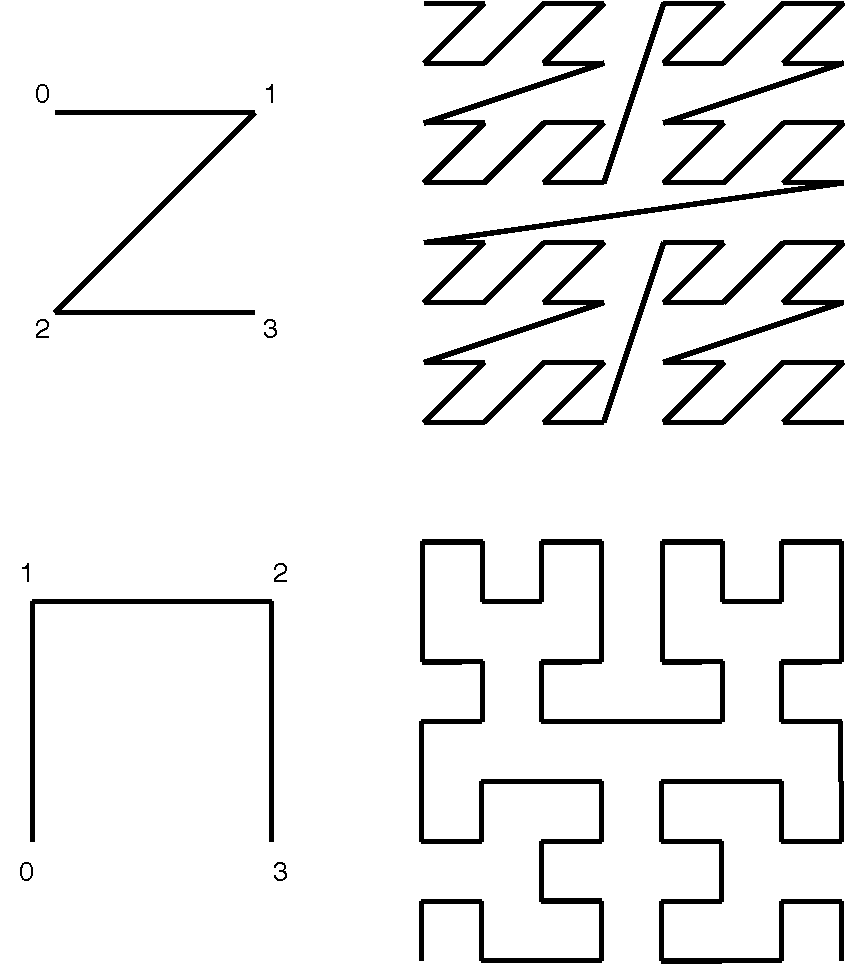
\includegraphics[scale=0.5]{Figures/space_curve.pdf}
\caption{Z-ordering Curve and Hilbert Curve}
\label{fig:space_curve}
\end{figure}

\paragraph{Z-ordering Curve}
Z-ordering \cite{Orenstein:1984jq} is a space filling curve dynamically hashing points that are close to each other, which is based on the Peano curve. The process of obtaining a z-ordering curve on a space starting from splitting into two equal sized subspace by ${(d-1)}$-dimensional hyperplane. This process can be executed recursively until it meets the following criterias \cite{Gaede:1998fp}. 

\begin{itemize}
    \item The current subspace does not overlap the data object.
    \item The current subspace is fully enclosed in the data object.
    \item Some given level of accuracy has been reached.
\end{itemize}

Each subspace can be represented by a unique z-ordering hashed bit string. To construct z-ordering bit strings in a coordinate system, one uses a bit interleaving the two binary values from the coordinates. For example, a value from a coordinate system can be represented as $(1, 2)$, the binary string for the two values is $001$ and $010$ respectively. The first value in the bit string comes from the first bit of the first value 1, followed by the first bit of the second value $0$. Therefore the first two bits are $01$, and the completed resulting bit string is $001001$. Z-ordered values created from the procedure are visually connected by a recursive z shaped curve. The resultant area collection is just an estimate of the initial entity. The accuracy and granularity (maximum number of bits) are required by the termination criterion. More Peano regions naturally will obtain more accuracy, but also sacrifice the size and complexity of estimating as a trade-off. The advantage of z-ordering is that spatial granularity shifts contribute directly to contextual improvements in the subsequent encoding. One drawback of z-hashing is that many useless data blocks will be created.

\paragraph{Hilbert Curve}
Another space-filling curve preserves locality well. Hilbert's order has been reported to be superior to the  Z-order curve as it has a better locality-preserving behavior \cite{Faloutsos:1991ue}. The Hilbert curve was first invented in 1891 by German mathematician David Hilbert \cite{hilbert1935stetige}. The fundamental idea is using a continuous line connecting the closest element in a grid, the difference between the Hilbert curve and the Z-order curve is that Hilbert is a U-shape curve. The transition from one column or row to the next is also choosing the closest cell rather than the diagonal cell in the Z-ordering curve. The U-shaped curve will be passed to the next cell in the grid in a similar manner, extending the continuous curve until the entire grid is filled in. The mapping of two-dimensional data stretches to the one-dimensional data layout, preserving the locality very well. It means that for points ${(x_n, y_n)}$ close to coordinates ${(x, y)}$, the output Hilbert value ${d_{x_n, y_n}}$ is also going to be closed to ${d_{x,y}}$. The Hilbert curve has been applied to the R-tree, combined with overlapping regions technique to improve the search performance. The Hilbert R-tree will be discussed in the latter part of the review. 



\subsection{Overlapping Regions}
Overlapping regions is a method that allows data buckets to access regions that have shared overlapped subspace. The linear transformation made point queries easier, but it is a challenge for handling range queries and containment queries without a complex spatial structure. However, redundant data can be created in overlapping regions, as a result, the number of search paths will be increased. Each insertion of new data can increase the overlapping area, eventually, overlap becomes too large for index searching efficiently. Therefore performance can be an issue for overlapping regions.

\subsection{Clipping}
Clipping has to be mutually disjoint, which does not allow overlapping between subspace. Consequently, the search path will only run through one path to the corresponding nodes instead of searching for multiple paths in overlapping regions. The major problem with clipping is also related to the insertion of new data. For new data that spans outside of the existing bucket region, a subdivision is required for subspace partitioning. This leads to a problem where more than one bucket has to be created for the same entry. The redundancy \cite{Orenstein:1989wy} can increase in the average search time, and also increase in the frequency of bucket overflow. Another problem with clipping is that when inserting new data, it can cause enlargement of the region if the region did not cover it. In certain circumstances, it is impossible to construct an enlargement without having an overlap between bucket regions. A new region has to be created due to overlapping is not allowed. This can potentially produce a much more complicated structure and problems with handling bucket insertion and overflow. Finally, due to splitting into smaller regions, the number of splitting regions will be increased. Hence, the database size is more likely to be large. 

\subsection{Multiple Layers}
Multiple layers \cite{Gaede:1998fp} are similar to overlapping regions, since regions in different layers can be overlapped. A hierarchical structure is usually used to combine with the multiple layers. However, data regions within a layer are disjoint, and it does not support extension to accommodate data objects. To insert a new data object, we attempt to find the lowest layer in the hierarchy structure that does not require to split. If such a layer exists, the data object will be inserted into that layer. If not, a new hyperplane will be introduced in order to split the new data region, then insert the data object to the new data region. Object will be moved to a higher layer, if it intersects the hyperplane. As we inserted more data into the structure, the higher layer will be collected on the higher layer, and the lower layers will have more segments of data objects. This can be inefficient for certain data distributions. Although, multiple layers still have advantage on selectivity of search path because of reduction of overlapping. 



\section{Traditional Spatial Data Indexes}

Characteristics of multidimensional data is complex  \cite{Gaede:1998fp, Robinson:1981id}. Gaede and Robinson have summarized some requirements for spatial indexes: dynamic, secondary storage management, a broad range of supported operations, independence of input data, simplicity, scalability, time efficiency, space efficiency, concurrency and recovery, minimum impact. The following sections introduce some of the popular traditional spatial indexing methods,  illustrate a wide range of techniques, as mentioned above, addressing the requirements for spatial index. 




\subsection{Grid File}

\begin{figure}[ht]
\centering
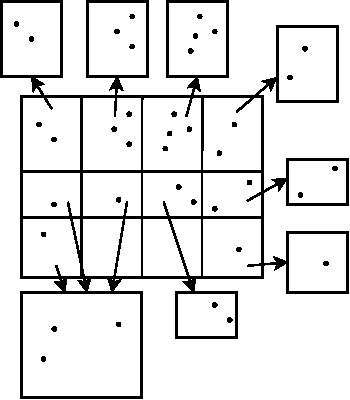
\includegraphics[scale=0.75]{Figures/grid_file.pdf}
\caption{Grid File}
\label{fig:grid_file}
\end{figure}

The grid file \cite{NievergeltJ:1984kc} is a hashing-based spatial access method, which is a grid layout partition to store data objects. A grid file consists of a rectangular d-dimensional cell, each grid cell has a number of shapes and sizes. A bucket contains one cell and many its neighbouring cells, and each cell is bound to one bucket. The main structure of the grid file consists of $d$ one-dimensional arrays called scales that are kept in the main memory. 


To perform an exact point match query, the first step is to access the location of the cell in the scale. Then the located cell will redirect to the reference of the page that contains all the potential points in that cell to perform an exact point match. The exact match query for the grid file is guaranteed to have 2 disk accesses. However for a range query, we must scan all cells that contain in the search region. 

Inserting a point to the grid file, the exact point match is also required. The matching query is trying to locate the cell, the point can be inserted if there is enough space. Otherwise we need to test if there is a hyperplane in the scale usable for separating data sections. When there is such a hyperplane a new data page must be generated and the data distributed accordingly. When no other hyperplane occurs, it would produce a splitting hyperplane. A new data page will then be generated, and the newly inserted point will be spread among the new data with the old data page. 


One of the major problems with grid files is dictionary split is expensive in high dimension, and even for uniformly distributed data it still has a super-linear growth of the directory. Some variations of the grid file tend to improve the structure and occupancy in the data buckets. EXCELL split the cell all in equal size, compared to the arbitrarily splitted space in the original grid file. The Two-Level Grid File added a level of grid file, limiting the splits without impacting too much of their surroundings to the subdirectory regions. The Twin Grid file introduced a second grid file parallel to the first one, which is a multilayer structure. The grid file has to create new data space by splitting thought hyperplanes when the number of points exceeds the limit. The twin grid file creates a new data space that requires redistribution of the data. 


\subsection{Multidimensional Linear Hashing}
MOLHPE proposed by Kriegel and Seeger \cite{Kriegel:vw} a multidimensional linear hashing with partial expansions to maintain order. This arrangement is based on the concept of extending the buckets in part without necessarily increasing the file size. Page address splitting depends on the page size from 0 to N, and a pointer p keeps track of the page. Two important contributions in building access methods. Firstly, whether a document remains in the old page or shifts to the new page only relies on the data key. Secondly, the old and the new sections will be filled in uniformly. Pages are united into groups to achieve a more evenly distributed loading factor. A group of pages will be expanded by one page once a new page has been added to the file. The file page expansion using an expansion pointer ${ep = (ep_1, \dots, ep_d)}$, and the address of the group is given by ${G(ep)}$. The expansion pointers will be updated along group partial expansion. 

It performed well over uniformly distributed data, outperformed many other spatial data retrieval systems. It overcomes the superlinearly growth of dictionaries in some multidimensional hashing methods such as the grid file. However, it does not handle very well on the non-uniform data distribution. A year later the same writers suggested linear order-preserving (PLOP) hashing to improve the performance on the non-uniform distributed data. The space partitions in PLOP are similar to the grid file, hyperplanes are organized by the binary tree. The d dimensional binary tree is also kept in the main memory just like the scale in the grid file. All the entries are stored in the leaf node, each leaf node from the binary tree is linked to each other for speedup.  




\subsection{K-D-Tree}

\begin{figure}[ht]
\centering
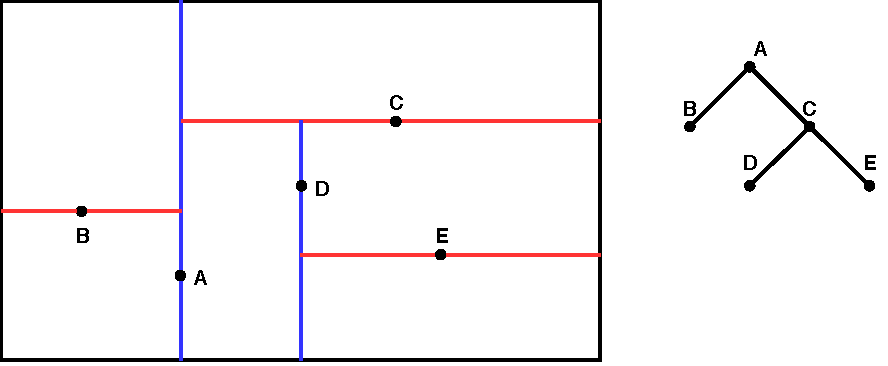
\includegraphics[scale=0.75]{Figures/kdtree.pdf}
\caption{K-D-Tree}
\label{fig:kdtree}
\end{figure}

K-D-Tree \cite{Bentley:1975gn} is a popular multidimensional data scheme that uses a hierarchical structure. It is a binary search tree, and each node represents a point in ${K}$ dimensional space. The universe of ${K}$ dimensional space is splitting by ${K-1}$ dimensional hyperplanes recursively. Each data point is used as the coordinate of splitting hyperplanes, which depends on whether the node is X-align or Y-align. The X-align or Y-align decides which axis to compare for newly inserted data points. The intermediate nodes have one or two descendants for search. The searching procedure is straightforward, comparing the corresponding axis value from the tree level, then going to the right or left subtree, repeating the process until the goal data point is found. 

One of the problems with the K-D-Tree is that the order of inserting points can have a large effect on the shape of the tree. Also, data points are distributed scattered over the tree, which will be difficult to execute complex queries such as the nearest neighbours query. Keeping the tree balanced can also be hard since the structure of the tree is mostly decided by the order of insertion. 

The adaptive K-D-Tree \cite{Bentley:1975gn} improves on the splitting by choosing the point that between points are evenly distributed on both sides. The splitting point is no longer taken from data points, data points are only stored in the leaves. Intermediate nodes store the coordinates of splitting points and the dimension information. It improves the original structure trying to store point values evenly, but it is still sensitive to the order of points being inserted. 


\subsection{BSP-Tree}

\begin{figure}[ht]
\centering
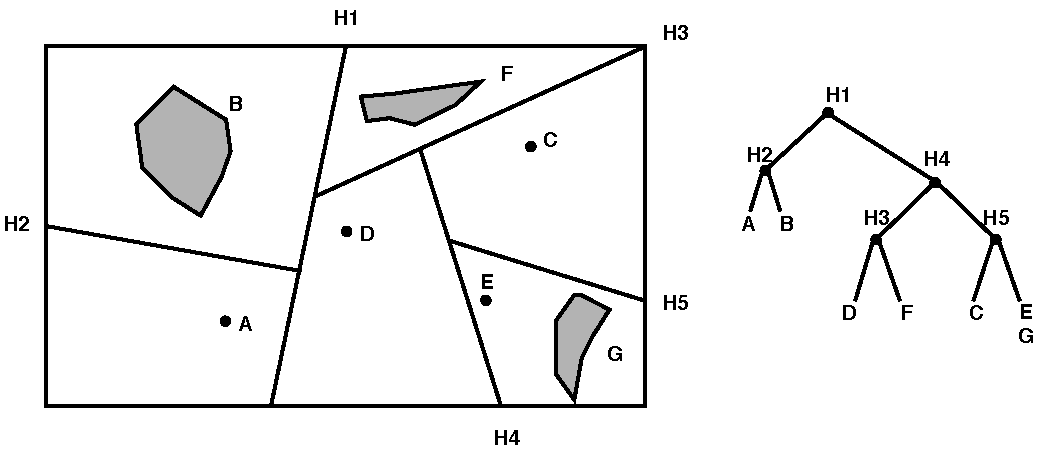
\includegraphics[scale=0.75]{Figures/bsptree.pdf}
\caption{BSP-Tree}
\label{fig:bsptree}
\end{figure}

Comparable to K-D-Tree, the BSP-tree \cite{Fuchs:1980bj} is also a binary tree with a recursive subdivision subspace by splitting hyperplanes. Instead of vertical or horizontal lines in the K-D-Tree, the BSP-tree uses the arbitrary orientation of splitting hyperplanes. It allows the subdivided space to be more flexible and well suited for arbitrary shapes of spatial objects. Since data points are not used as the splitting hyperplane, each subspace can be divided independently. The partition hyperplane can be selected depending on the distribution of data objects. 
Inserting a point to the tree is also similar to the K-D-Tree. Starting from the root node, the search point has to compare with the value in the root node and determine whether to go to the right or left part of the tree. All data objects are stored in the leaf node, so the search will stop until reaching the leaf node of the tree. 
The BSP-Tree can handle non-uniformed distributed data well. However, arbitrary splitting hyperplanes also require more complex calculations and storage space. 



\subsection{Quadtree}

\begin{figure}[ht]
\centering
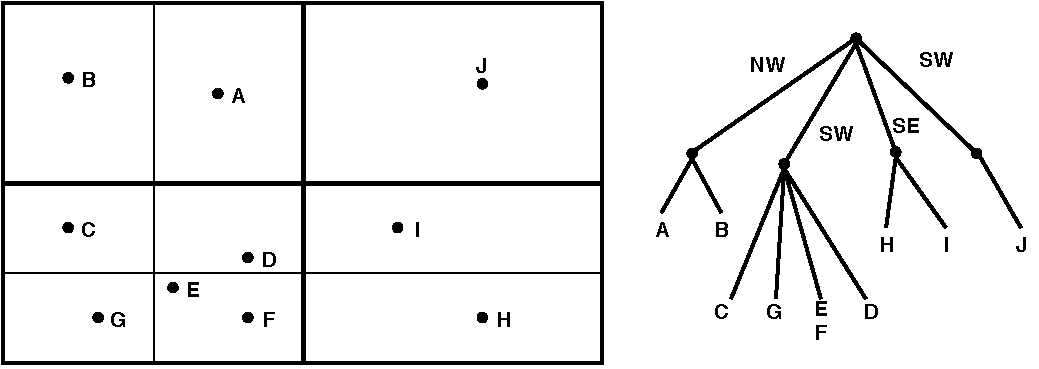
\includegraphics[scale=0.75]{Figures/quadtree.pdf}
\caption{Quadtree}
\label{fig:quadtree}
\end{figure}

The Quadtree \cite{CSUR:tm} is also considered to be closed to the K-D-Tree. The difference is the Quadtree is not a binary tree anymore. The intermediate node in the Quadtree will have ${2^d}$ descendants for d dimension. For example, d=2 will have four descendants, which each of the descendants is referred to as a rectangle region. These four descendants can be viewed as quadrants that represent four directions(NW, NE, SW, SE) prospectively. The recursive subdivision will be continued on the rest of the data. Consequently, the Quadtree will not be balanced since that more densely the region is deeper the tree will grow. 

Searching and inserting in the Quadtree is similar to other tree structures. New data points will start from the root node, the node will decide one subtree from the four descendants. For point query, there always will be only one candidate subtree for further searching. For range queries, there might be one or more candidate subtrees. The process will continue recursively until finding the goal.


\subsection{R-Tree}

\begin{figure}[ht]
\centering
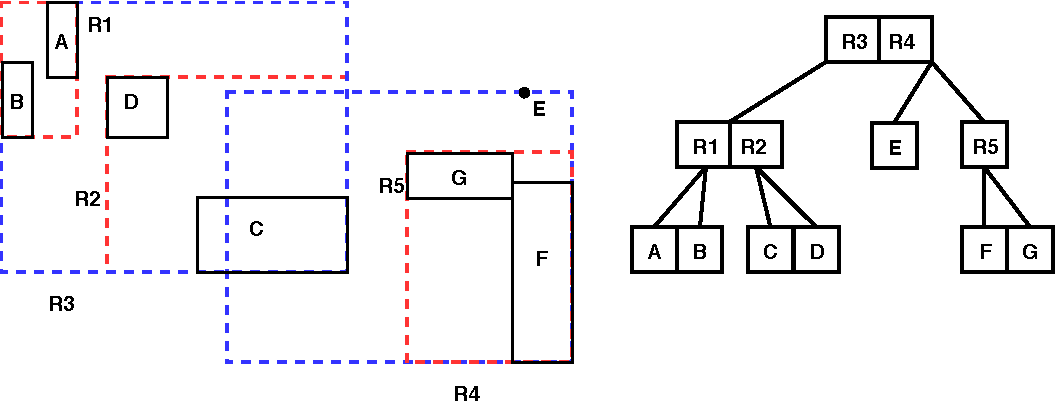
\includegraphics[scale=0.75]{Figures/rtree.pdf}
\caption{R-Tree}
\label{fig:rtree}
\end{figure}

R-Tree\cite{Guttman:1984ka} is a height-balanced hierarchical data structure that applies overlapping technique. Only the leaf nodes store the minimum bounding box (MBB) of data objects. For the interior nodes, each node has to store two information: children of the node and a MBB that contains all the nodes. The R-Tree contains the following properties: 

\begin{itemize}
  \item Each leaf node contains between m and M index records, except the root node. 
  \item For each entity in a leaf node, a minimum bounding box is used to contain the n-dimensional data object.
  \item The root node has at least two entries unless it is a leaf.
  \item All leaves are at the same level.
\end{itemize}


The increase of branching factor ${m}$ will decrease the tree height and improve space utilization because most of the space will be used in the leaf nodes. Searching in R-Tree is similar to the B-Tree. At each node in the tree, they will be tested if within the search ranges. Since the bounding boxes in R-Tree can be overlapped, the search path can go through more than one subtree. Because R-Tree only stores MBBs, the search result is not an exact match result. For actual spatial context data, we need to search further within MBBs.

Insertion in R-Tree is also similar to B-Tree. The newly inserted object first recursively finds a path to the leaf node starting from the root node. If the leaf node is not full, insert the new object. Otherwise, the leaf node has to be split by a splitting heuristic. The old objects from the original node will be distributed among the original and new nodes. We can adjust the tree by propagating the newly added nodes up and change the height of the tree. 

For the deletion of a node in the tree, the search query must be performed. If found in a leaf node, then delete it from the node. If there is not an underflow, the MBB will resize according to the updated nodes. If it causes an underflow, and the node occupation below ${m}$, then adjusting the tree is needed, the subtrees of the node will be dissolved and these nodes will propagate upwards. Old entries in the node will be inserted into a new temporary node or another option is to merge with siblings node. In both options, the tree has to adjust the MBB size and propagate upwards. 

To reduce the overlaps in insertion, the author proposes several different splitting algorithms in the original paper. A quadratic-cost algorithm picks two of the M+1 entries as the first elements of the two new groups. The criterion of choosing the pair is that they would take most areas if both were put in the same group, which means the region of a rectangle covering the two entries, minus the region of entries themselves, would be the largest. A linear-cost algorithm is similar to the quadratic-cost algorithm but uses different criteria to select the two entries. The two entries were selected based on the dimension of entries. For entries whose highest low side and lowest high side, record such separation. The separation will be normalized by the width of the entire set along the corresponding dimension. Then choose the pair with the greatest normalized separation along any dimension. 

\section{Learned Indexes for One-dimensional data}
\subsection{The Recursive Model Index}
 Kraska \cite{Kraska:2017vh}  proposed a method that uses a machine learning model to replace indexes. Kraska introduced the idea that data indexes can be treated as models, we can describe the data distribution by constructing the cumulative continuous functions. A B-Tree indexes a key into a hierarchical structure, retrieving the position of that key from traversing the tree. It stores as many as children as possible to diminish the height of the tree, hence to reduce the number of disk access. The B-Tree is a self-balance tree, it only provides an approximate position with min and max error with stored keys. The optimal searching time complexity requires log time retrieval. To insert and delete a key, B-Tree needs to re-balance to provide the same search time guarantee. More importantly, strong error bounds are not needed since prediction results can be replaced by local precise search algorithms. Identical patterns obtained in a continuous function that used to describe a distribution of data can be used to build a data structure for indexing. As a result, range searching in the B-Tree index can be replaced by machine learning models such as linear regression, which can predict an approximate point to the next stage and error from the prediction does not affect the final search accuracy. 

\[p = F(Key) * N\]

The CDF models data distribution and predicts the position of the key as shown above. P is the predicted position, F is the cumulative distribution function estimate likelihood for a range observed key and N is the total number of the key. The learned index is optimized by learning the CDF and minimizing the error from the linear regression model. The recursive-model indexes (RMI) is a series of machine learning models on a hierarchy structure. The RMI consists of multi-stages, where the model predicts a value from the input key at each stage. Due to range indexes that can point to a range of values, the predicted value does not need to be exact. The predicted value can be the final position result if at the final stage of the structure or a pointer to the next stage if it is not the final stage. 

In the experiment, the recursive model can be built by a mixture of machine-learned index models and B-Tree. For a 2 stage model: the top stage is a 2 layer fully-connected neural network with 32 neurons per layer with the ReLU activation function, and the second stage can be thousands of simple linear regression models or B-Tree. The data distribution learned by the model can give a prediction of the pointer, the pointer is pointing to a specific range of values in the next stage. All models at final stages are trained by a specific range of values, and have much better accuracy for values within that specific range. In other words, we are reducing the searching range of values at each stage. However, like most neural net models, the prediction value can have uncertainty with min-/max-error. In the case of the neural net model performing worse than a threshold, the neural net model can be replaced by a B-Tree to ensure the ‘last-mile’ accuracy. 

Two search strategies mentioned in the paper, one is the model biased search and another is biased quaternary search. The model biased search is a simple binary search that it set the middle point of as the predicted value from the model. Tha biased quaternary search takes ${pos - \sigma}$, ${pos}$, ${pos + \sigma}$ as the initial three points, which can make the initial guess as accurate as possible. The min- and max-error sets upper and lower bounds that can guarantee all the points can be found. However, a wrong lower or upper bound can be generated for non-monotonic RMI models if the key does not exist. 

Kraska also discussed some applications of the learned model on other data structures.  The learned hashmap is trying to use a CDF to replace the hash function. The result shows the learned hashmap can reduce the number of conflicts by up to 77\% on a certain dataset. Kraska suggests that for a uniform distributed dataset, the linear model is no better than a randomized hash function. For small keys, traditional hash functions with Cuckoo hashing provide the larger payload and reduce conflicts from distributed hashmaps. 



\subsection{ALEX}
The ALEX \cite{Ding:2020wo} is an adaptive learned index improvement of the RMI. The major improvement is that ALEX uses different data structures to store data on the leaf nodes, whereas RMI uses only one single array. Gapped Array (GA) and Packed Memory Array (PMA) are the two node layouts that have been explored in the paper. Since all the data are stored in the leaf node, the search method in ALEX uses exponential search. The other feature is that ALEX adjusts the shape and height of the RMI dynamically depending on the updated workload. It also inserts records dynamically, which stores the key at where the model predicts. 


Gapped Array is one of the node layouts that use the idea of exchanging extra storage for the speed. It creates a gap during insertion to maintain good exponential search, then utilize the gaps with adjacent keys. To insert a new key into a gapped array, we must find the insertion position. RMI is used to predict the insertion position, if this insertion position is maintaining the sorted order, and is a gap, then the new key is placed to the gap and finish. If the predicted insertion position is not right, we have to use an exponential search to find the correct insertion position. The correct insertion position must be a gap to insert the new key. If it is not a gap, we shift the elements at this position by one position in the direction of the closest gap. The insertion performance achieves ${O(logn)}$. One procedure during insertion is if a new key pushes into the gapped array and exceeds the density bound ${d}$, then the gapped array needs to expand. A disadvantage of gapped arrays is when inserting a long contiguous region without any gaps, such \emph{fully-packed region} can cause a dramatic increase in the insertion time. 

Packed Memory Array is another node layout that has been shown to adopt and grow better to insert. The PMA is an array whose size is always a power of 2, and it divides itself into powers of 2 numbers of segments. The PWA builds an implicit binary tree, each segment is a leaf node and the root node represents the entire array.  Each node will have a density bound that can determine the maximum number of elements to the position in the region of the array. The size of PWA will expand once the density in the array becomes too full. The rebalance local portions of the PWA allows data to be uniformly distributed. 

Adaptive RMI Initialization in ALEX sets a predetermined maximum bound for the number of keys in a leaf node so that ALEX can determine the RMI depth and the number of leaf models adaptively. The root node will be divided into a certain number of partitions, and each partition will have exactly the maximum number of keys. Node splitting on inserts is another optimization in ALEX. If the new key will push to the leaf node exceeds the maximum bound, then we can split the node. The corresponding leaf node will become the interior model, and a number of children nodes will be created from the model. This allows the ALEX to start with empty data, and the RMI will grow deeper along with more inserted nodes.


\subsection{The PGM-index}
The Piecewise Linear Approximation model \cite{Ferragina:ud} is a pure learned data structure, rather than a hybrid learned model such as RMI. The PGM-index builds upon a sequence of segments, each one indexing a sequence of keys in constant space and constant query time to return the approximate position of the key in the array. Another property of the PGM-index is it is a recursive algorithm that constructs the index structure to fit the distribution of the keys. 

The PGM-index is to focus on optimizing space-time trade-off. It has the following advantages in space-time complexity:

\begin{enumerate}
    \item Since the PGM-index is built upon the minimum number of segments from bottom-up, which is more efficient than other learned indexes in terms of time and space. 
    \item The PGM-index uses these segments as a constant-space routing table, rather than storing large number keys depending on the disk-page size in other learned indexes. 
    \item The routing tables in the PGM-index take constant time to limit the search of a key in a node to a smaller subset of the indexed keys.
\end{enumerate}

 The author provides compression algorithms to reduce the number of distinct slopes to their optimal minimum number for the compressed PGM-index. The multicriteria PGM index exploits the space-time flexibility by optimizing in two different criteria: 
\begin{enumerate*}
  \item Given a space constraint the output PGM that minimizes the query time.
  \item Given a maximum query time the output PGM that minimizes the space.
\end{enumerate*}
The number of $\varepsilon$-approximate segments controls trade-off between the space and time. The space occupancy decreases with increase of $\varepsilon$, whereas the query time ${t(\varepsilon)}$ increases with increase of $\varepsilon$. 

The performance result shows that the PGM-index improves space occupancy by offering theoretical bounds, and it guarantees a 4X increase in the precision of the estimated position of the searched key compared to the RMI. The PGM-index is reported to provide better latency guarantees since it can dynamically adapt to the data distribution, and it can use the ${\varepsilon}$-approximation to optimize a better performance trade-off between space and time.


\subsection{RadixSpline}
RadixSpline \cite{Kipf:2020wr} is another learned index that builds upon a single pass over the data. RadixSpline is built in a bottom-up approach in two steps. First, a linear spline is to model the cumulative distribution functionc (CDF) of the data, which guarantees certain error bounds. Second, a radix table will be built as an approximation index into the spline points. 

To build a RadixSpline, we first construct an error-bounded spline model $S$ on top of the underlying data. The spline model $S$ always predicts the correct location of the data within a constant error of $e$. The parameters of the model $S$ are a set of spline data points $Knots(S)$. For any look up key $k$, linearly interpolating between the two closest spline points in $Knots(S)$ will output an estimate within error $e$. 

Then, the selected spline points are built to index in a radix table. The radix table can quickly find the two spline points surrounding the lookup key. It is a flat $uint32_t$ array that maps fixed-length key prefixes (“radix bits”) corresponding to the first spline point. The radix table uses $r$ as a parameter, so array size will be ${2^r}$. To increase the precision, the size of the array ${2^r}$ will grow exponentially with growth of $r$. The RadixSpline supports single pass building CDF, that means the sorted data points are passed in the spline construction and radix table allocation at the same iteration. 

Lookup in the radix table takes following procedures: first to extract an $r$-bit radix prefix $b$ from the key. Then, we can use the $b$ radix prefix access to the radix table retrieving two spline points. A linear interpolation will be performed between two spline points to find an estimated position $p$ of key. Finally, it uses a binary search to find the first occurrence of the key within the error bound $(p \pm e)$

The building performance of RadixSpline is significantly lower than the RMI. In lookup latency, RadixSpline performs similarly with RMI, which both are better than traditional indexes such as B-Tree. However, the lookup latency of learned indexes can be affected by the distribution of the dataset. The index size of RadixSpline is unstable for different dataset, the paper reports significantly high memory cost in one of the dataset. 

\subsection{FITing-Tree}
FITing-Tree \cite{galakatos2019fiting} is another learned index that uses a piecewise linear function for key index approximation. The idea of the FITing-Tree is to partition keys into fixed-sized segments within certain error bounds. The error is defined as associated with the maximum prediction error distance between the actual position and the predicted position. Two types of FITing-Tree have been proposed, which a clustered FITing-Tree manages sorted and indexed key in table pages, and a non-clustered FITing-Tree adds an “indirection layer” to store sorted pointers to the key. 

Lookup and insert of the interior nodes in a clustered FITing-Tree are similar to B+tree, but once the operation reaches the leaf node, the FITing-Tree does some additional work. The FITing-Tree stores a segment's slope, starting key, and a pointer to a segment at leaf level. Linear interpolation calculates the approximate position from a given slope. 

The major difference between a non-cluster and a cluster FITing-Tree is the additional “indirection layer”. This layer indexes an array of pointers to the values that have been sorted within each segment, while the actual data remains unsorted in the table pages. All operations in the non-cluster FITing-Tree are performed on the indirection layer. To look up a data item, it must find the index of the pointer to the query data item in the indirection layer first, then the pointer returns the actual position in the table pages.

Besides point query, FITing-Tree also provides range queries. For a given start or end of a range in the tuple, the searching node performs a tree traverse to the leaf, where it stores the slope and starting key of the segment that can be used for index prediction. Since values in the clustered FITing-Tree are sorted, and the pointers are also sorted in the indirection layer in the non clustered FITing-Tree. The search can take place contiguous until reaching the end of the range. 


Similar to other learned indexes, FITing-Tree requires local search at leaf nodes. The clustered method requires sorted data, while the non-clustered method doesn’t require data to be sorted at table pages but pointers in the indirection layer still need to be sorted. The reported result \cite{galakatos2019fiting} showed that a non-clustered FITing-Tree is smaller than a non-clustered B+ tree with fixed-size pages because of fewer leaf and interior nodes that it has. 



\section{Learned Spatial Indexes}
\subsection{Learned ZM index}
Inspired by the Learned Index, Wang \cite{Wang:2019ks} integrate the idea of using models to replace indexes and spatial technique to create an index model for spatial queries. One of the difficulties of the multidimensional access method contrasts with one-dimensional is to preserve the sequential order of spatial indexes. Learned spatial index can adopt a similar idea from one dimensional learned index models. The concept of the Z-order curve can help to convert multidimensional data into 1D space vectors. By interleaving two bit strings x and y from a coordinate point (x, y), we can generate a unique number for this point on 1D vector space, which is referred to as Z-address. The multi-staged recursive model is similar to the Learned B-Tree model, using the predicted value as a pointer to access to models at the next stage. This can guarantee the lower bound of the error from the model prediction will not propagate to the next model. 

The search strategy for range query processing is based on Model Biased Search (MBS) proposed in \cite{Kraska:2017vh}, which is different from the pointer approach in the B-Tree model. It is similar to binary search except that the first middle point is set to be the predicted value from the model.  The MBS is to find the precise position of the data object after the RMI predicts the estimated position.

The Learned ZM index is reported to save above 90\% memory compared to R-Tree since the structure itself only has a few parameters instead of storing data objects. The Point query performance of the ZM is 2.3X and 2.5X of the R-Tree on the two dataset RANDOM and POST respectively. For the range query, the performance is varying from selectivity from 0.0001 to 0.1. The ZM performed better than the R-Tree when the selectivity is low, but R-Tree has slightly fast query time when searching in a larger range of selectivity. 



\subsection{Recursive spatial model index}
The recursive spatial model index (RSMI) \cite{Qi:2020uz} is another spatial data index that incorporates the Z-order curve and the RMI. Data points in the spatial space are first mapped to a $n \times n$ grid to describe the rank space. Then a Z-order curve maps every point on the rank space with a curve value. All points are sorted in ascending order based on the curve value, then points can be packed into a block by $p.blk = [p.rank \cdot n/B]$, where B is the capacity of a block. Then, a regression model is trained to predict the $p.blk$ for given point coordinate. 

For a larger scale data set, the RSMI partition all data points into a certain size of the grid. Each of the grid cells contains up to a certain number of data points. At the top level, the model is predicting a value that is not directly the exact matching result. Then, we can regroup points with the same block curve value. The partition will be repeated to follow in the same manner, the learned model in each partition predicts which sub-partition the point belongs to. Once the partition is completed, data points along with block id from preceding and subsequent blocks are stored in each block. The pointer of block id makes it easier for access and searching in blocks at a different level. 

To execute a point query in RSMI, the coordinates of the searching point is used as the input query that can be fed into the learned model. The searching process is done recursively, starting from the root model, the prediction value is pointing to the submodel at the next level. The searching procedure is repeated recursively until reaching the leaf model. The output prediction value from the leaf model is the block ID of the input point. At the final stage, we can examine the block and its neighbouring block within an error bound. 

For the range query, we can locate the minimum and maximum curve value $q_min$ and $q_max$ from the input query. Then it retrieves all the candidate points between $q_min$ and $q_max$. Finally, candidate points can be filtered out from the window range, and remaining points will be the result. 

The K nearest neighbour query in RSMI starts with searching in a small region around the input query key. It will keep searching in the expanding region until $k$ points are found. A window query will be performed when the search region is expanding. Measuring the distance from the point to the query point, and comparing to the existing points that have the minimum distance in the result. The initial search region size can be determined by the number of points and number of regions for the uniformly distributed data. Two skew parameters are introduced to adjust the search region based on the skewness of the data. 

The result shows that the RSMI has a good performance on the point query, the number of block accesses is significantly lower than traditional data indexes and the ZM model. A disadvantage of the RSMI is that the training time cost is much higher compared to the traditional methods. The training time of RSMI is also higher than the ZM model since sorting is needed for each partition.




\subsection{Flood}
Flood \cite{Nathan:2019wc} claims to be the first learned multi-dimensional in-memory index, which is based on the point access method grid file. The Flood model first to preprocess offline to choose an optimal layout for indexing, then an online component to handle executing queries. 

The model breaks down into three parts: Projection, Refinement and Scan. Similar to the traditional grid file, projection first to match a query is to locate the cell containing the search point, which is to identify the range of position in storage. Compared to z-address, points in the columns that are along x and then sorted by their y-values, creating the serialization order. Then, refinement can narrow down the range of search. When query overflows the sort dimension, Flood can take advantage of the ordering of points within each cell to further refine the physical index ranges. The final step is to scan and find the matched query filter. The model time complexity depends on the weight for each step $w_s$, $w_r$ and $w_s$ and size of cells and scanning points. 

Flood also uses a piecewise linear model(PLM) to train the CDF. By using PLM, the partition boundary between each column is not equally spaced. A flattened layout, as referred in the paper, is introduced to correlate with unevenly distributed data. They also mentioned that modelling based on a single-dimensional attribute was sufficient to reach an equal number of points in each partition. 

Compared to other traditional multidimensional data structures, Flood shows significant performance improvement on query time. In measuring varying query selectivity, Flood also works well and outperforms other traditional methods. 


\subsection{Tsunami}
A more recent study from the same authors of the Flood model proposed an improvement index Tsunami \cite{Ding:2020we} based on the Flood model. Flood has some limitations when training on the non-uniform data distribution, each grid cell can have uneven distribution of data points. To address this problem, Tsunami proposes a data structure composed of the Grid Tree and Augmented Grid. 

The Grid Tree divides space into partitions based on the values of split dimension. Each partition contains a number of data points, which are stored in the internal node of the Gird Tree. An optimization is applied to the Grid Tree to minimize the query skew, by setting the split value that reduces the skew the most. 

The Augmented Grid can correlate the points within each sub-region. Several different strategies can be applied to create partitions. Notably, the strategy used in Flood is $CDF$ on $X$ independently from other dimensions. It can use a conditional $CDF(X|Y)$ that X dependent on another dimension $Y$. It can also use a functional mapping to some dimension other than $X$. They used adaptive gradient descent to optimize the augmented grid for the lowest average predicted query time and search space size. 

The performance result shows that query time for Tsunami is 6$\times$ faster than Flood and 11$\times$ faster than the traditional index. The index size of the Tsunami is also much less than other indexes. The advantage of Tsunami is that it proposed strategies for data correlation to produce a more uniformly distributed data from a skewed dataset. There is still room for improvements, as mentioned in the paper, functional mapping can not handle outliers very well, the error bound can be enlarged; and the Augmented Grid can not handle higher dimensional data. 

\subsection{qd-tree}
Qd-tree \cite{Yang:2020ev} is a high-dimensional data space partitioning binary tree, which is similar to the k-d tree. The qd-tree approaches the query task from a deep reinforcement learning-based framework. The structure of the qd-tree is built upon the binary tree. Each node in the tree contains data records that belong to the multidimensional data. The root node of the tree holds all the information for the entire dataset. 

The strategy of querying entry in the tree is using a concept of routing data. Data is stored in the blocks on storage. Every record starts routing at the root of the tree, the same as most of the hierarchical structure, the record will recursively traverse down the tree. At each node, the tagged predicate $p$ is evaluated on the record. Each predicate in the node does range comparison ($\{<, \leq, >, \geq\}$) and equality comparison ($=$). A record at the node does a series of range comparisons to decide which leaf (left or right) to go.  Eventually, the record will be landed in the leaf node. The leaf node represents the physical location of the record on the disk. The block ID (\texttt{BID}) is stored along with the record on the leaf, indicating where the record belongs to. 

The Greedy approach is beginning with a single root node that contains all the nodes. Then iterate through all the nodes to split the leaf node that is larger than $2b$ into two children nodes, the size of each of the children nodes is at least $b$. The Greedy approach has been reported \cite{Yang:2020ev} to work well to reach the local optimum and may be global suboptimality. 

The Deep RL method is a black box learning process without assumption on the data distribution or query. The Deep RL agent Woodblock is built on top of the Markov Decision Process (MDP). It defines the state space to be any subspace of entire data space, and action space to be the set of splits. The Woodblock agent contains two parameterized networks: 
\begin{enumerate*}
    \item \textit{Policy Network}, which takes a state and emits a probability distribution over an action space.
    \item \textit{Value Network}, which estimates an expected cumulative reward for a given state.
\end{enumerate*}
The learning process trained through a series of episodes: 
\begin{enumerate}
    \item Starts from a node off from the queue,
    \item Evaluates the policy at current state,
    \item Choice an action from the output distribution,
    \item Applies this action on the current node to produce a new node.
\end{enumerate}

A stopping condition is necessary for ending the episode training. As it is defined in the tree structure that the leaf node must contain at least $b$ records, the agent will continue to make cuts on the current node if it contains more than $b$ records. Overlapping region existing in the qd-tree. To handle such data redundancy in the leaf node, qd-tree proposed a relaxed cutting condition that allows one of the children nodes to have a size smaller than $b$.  


\subsection{LISA}
LISA proposed by Li \cite{Li:2020ki}, designated to generate data layout that allows using machine learning models to search in an arbitrary spatial dataset that is stored in the disk pages. Similar to many popular traditional approaches, LISA partitioning space into a series of grid cells, and numbering the cells along a sequence of axes. It builds a learned regression model $SP$ to map the keys distribution into different shards, and assign an id for each shard. All shards preserve order concerning the corresponding interval in the mapped data. Keys in shards are stored in several disk pages, which means that one shard might contain keys from different pages. At the final stage, local models are required for page address lookup for the given query. 

LISA also adopted a piecewise linear function as the shard prediction function. The piecewise linear function is a monotonic regression model, and it allows the mapped values to be sorted. Therefore, the operations for searching members of different partitions at the bottom level is efficient. The range query in LISA access to the keys that belong to the search region. Similar to traditional spatial indexes that applied \textbf{overlapping regions} technique, since the space partition might divide keys from different disk pages, it has to scan the overlapped pages in local models. For a KNN query, the given point and the number of return values k, LISA will estimate the distance bound base on the query. Then, the keys remaining within the bound are selected to perform repetitive range queries, until we get K nearest keys. 

Compared to traditional such as R-Tree, KD-Tree, the advantage of LISA is that it benefits from the learned monotonic function. The learned monotonic function allows the mapping order of keys to be sorted, keys that to be appended to the structure are naturally sorted. Hence key lookup in neighbouring value and update handling in LISA is easy. Even though it still has overlapping regions in the local models, LISA still does less data updating than R-Tree. 

\subsection{ML-Index}
The ML-Index \cite{Davitkova:2020dx} is another learned index for multidimensional data, and it supports point query, range query and KNN query. The ML-Index consists of two main components, the first part of the structure is to convert and scale the two-dimensional data into one dimension, and the second part is to use an RMI model as mentioned above by Kraska to learn the CDF of the data distribution. 

The upper part of the algorithm is to scale a group of points that are similar to each other, and project into one-dimension. The first scaling method is to map distances of all points to a single reference point and use the distances as keys. It works for small datasets, but it is hard to scale to larger datasets. The second scaling method is called iDistance by Jagadish et al. \cite{jagadish2005idistance}, $key = i \times c + dist(O_i, d_l)$, where $i$ is the index of the closest reference point $O_i$, and a constant $c$ partitions the points into predefined ranges and stretches the range according to its value. The third method calculates the offset value as the scaling value $key = \text{offset}_i + dist(O_i, d_L)$, where the offset is calculated by sum of the radii of every partition that is based on their arbitrary reference points.  

The second part of the index is to build a recursive learned index as described in Kraska's paper. Instead of building multiple stages models in the original paper, the ML-Index uses only two stages to reduce expected error by increasing the number of models in the second stage. 

The point query procedure is the same as RMI, which uses scaled values to predict bounds containing the expected query result from $[pos - err, pos + err]$. The range query iterates through the reference points and calculates the closest and furthest point for each reference point from the query range. Then issue the model prediction to find keys that are within the range. For the KNN query, the algorithm first predicts the position of the query key to locating the starting point of the search. 


\subsection{PolyFit}
PolyFit \cite{li2020polyfit} uses piecewise polynomial functions to process approximate range aggregate queries. Aggregate functions including COUNT, SUM, MIN and MAX. The key cumulative functions are extracted from those aggregate functions. Then the measured key cumulative function is used to construct the index. 

The PolyFit index is built upon polynomial fitting for an interval of data. The polynomial function can achieve a better approximation of data distribution when compared to linear regression or piecewise linear regression. It is hard to fit the whole dataset with one polynomial function. Therefore, it also utilizes multiple polynomial functions to reduce the fitting error, which could get the approximate function more accurately. Memory consumption is also worth considering, one way is to use dynamic programming to minimize the number of polynomial functions while fitting the dataset well. Authors proposed Greedy Segmentation method (GS), it inserts one more key into the interval incrementally, then checks whether the interval can fulfill the bounded error constraint. 

The PolyFit can be extended for two-dimensional queries. Similar to the one dimensional range aggregate queries, it estimates the key cumulative function with two keys for COUNT query. Then follow the same idea from GS to utilize the number of polynomial functions. However, the GS method takes $O(n^2)$ to obtain the minimum number of segmentations. They use a Quad-tree based method to get the segmentations. If a segmentation does not fulfill the error guarantee, the space partition can be continuously broken into four smaller partitions. 



\section{Research Gaps}
Researchers have different perspectives on constructing access methods for multidimensional data, from a traditional hierarchical structure to a learned index. 

The learned index is opening a new page for traditional data access methods by applying machine learning. The optimization of the machine-learned model seems to have a big advantage over traditional hierarchical methods. The complexity of the model is scaled by the width $h$ of the model and input length $N$: $O(hN)$. The linear model only using multiplication and addition operation: $w*x+b$, to calculate the prediction value. As a result, the Learned Index does not have searching phrases between stages. Consequently, it can achieve constant searching time complexity, while hierarchical structure B-Tree requires $O(logn)$ searching time. On space complexity, the learned index also has an advantage over B-Tree. For inserting a new key, we might not need to re-train the entire model depending on the key. The new key could fall into a range at the next stage, the root stage model can predicate the same pointer to the next model that has the same range of keys. 

However, there are some drawbacks to the learned index. For indexing, finding the min and max error of a position is more interesting to us. A typical machine learning model is to generalize the result, make it more suitable for real-world data. In the learned index, we wish to minimize the error as close to 0 as possible to achieve accurate results. It is different from a data science aspect problem, the fitting curve is preferred to overfit the dataset instead of generalizing the model. 

The neural net model at the top stage does not produce the exact position of the key, requiring a 'last-mile' searching phase. The accuracy problem still exists in the ‘last-mile’ phase, which means the model still relies on hierarchical structure and traditional indexing method. The B-Tree is cache efficient. Machine learned models require all weights to compute a prediction, in which the multiplication and addition cost more memory. 
 

Both Wang \cite{Wang:2019ks} and Nathan \cite{Nathan:2019wc} represent multidimensional spatial data in a linear vector space. One of the difficulties of spatial data is the consistency of simultaneity ordered on different dimensions. For example, on a 2D spatial data, the growth of the Y-axis does not grow simultaneously along the X-axis. 


The learned ZM index is trying to solve multidimensional problems in a one-dimensional way. The z-order curve or z-address is aiming to solve the consistency of simultaneously ordered spatial data on different dimensions. Interleaving bits of two-point value in a coordinate can convert the multidimensional data into one dimension. Applying the learned index model from Kafle \cite{Kafle:2017dy}, we could achieve a similar result as the learned B-Tree model. 

The advantage\cite{Ding:2020we} of the Flood is that the query performance can be boosted by automatically adjusting the number of partitions in each dimension. The more partitions in the data space, the fewer points are needed to be scanned. A drawback of Flood is that it is not optimized for skewed data. For a query that is non-uniform, it will scan a large range of points until reaching the result. 


\begin{adjustbox}{width={\textwidth}, totalheight={\textheight},keepaspectratio}%
\footnotesize
\newcommand*\rot[1]{\hss\rotatebox[origin=br]{-60}{#1}}
\newcommand*\rotNarrow[1]{\hbox to2em{\hss\rotatebox[origin=br]{-60}{#1}}}
\newcommand*\feature[1]{\ifcase#1 -\or\LEFTcircle\or\CIRCLE\fi}
\newcommand*\f[5]{\feature#1&\feature#2&\feature#3&\feature#4&\feature#5}
\newcommand*\ff[6]{\feature#1&\feature#2&\feature#3&\feature#4&\feature#5&\feature#6}
\newcommand*\fff[8]{\feature#1&\feature#2&\feature#3&\feature#4&\feature#5&\feature#6&\feature#7&\feature#8}
\newcommand*\ex[4]{#1&\ff#2&\f#3&\fff#4}

\begin{threeparttable}
\caption{Comparison of Data Indexes}
\label{tab:features}

\begin{tabular}{@{}l c@{}c@{}c@{}c@{}c@{}c@{} | c@{}c@{}c@{}c@{}c |  c@{}c@{}c@{}c@{}c@{}c@{}c@{}c}
\toprule
    Index Type
    & \multicolumn{6}{c}{Traditional Spatial Indexes}
    & \multicolumn{5}{c}{Learned Indexes} 
    & \multicolumn{8}{c}{Learned Spatial Indexes}\\
\midrule
% rotated items
 Model Name
 & \rot{Grid File}
 & \rot{MOLHPE}
 & \rot{K-D-Tree}
 & \rot{BSP-tree}
 & \rot{Quadtree}
 & \rot{R-Tree}
 %
 & \rot{RMI}
 & \rot{ALEX}
 & \rot{PGM-index}
 & \rot{RadixSpline}
 & \rot{FITing-Tree}
%  & \rotNarrow{PolyFit}
 
 %
 & \rot{ZM}
 & \rot{RSMI}
 & \rot{Flood}
 & \rot{Tsunami}
 & \rot{qd-tree}
 & \rot{LISA}
 & \rot{ML-Index}
 & \rot{PolyFit}\\

\midrule
\ex{Top-down Construction} {222220}{22000}{22220222} \\
\ex{Bottom-up Construction} {000002}{00222}{00002000} \\
\ex{Single-pass Training} {222221}{00020}{00000000} \\
\ex{Linear Structure} {020000}{00010}{00000000} \\
\ex{Hierarchical Structure} {002222}{22202}{22002022} \\
\ex{Grid Layout} {200000}{00000}{00220201} \\

\midrule
\ex{CDF approximation} {000000}{22222}{22222222} \\
\ex{Piecewise Linear Model} {000000}{00202}{00200200} \\
\ex{Recursive Model} {000000}{22202}{22000022} \\
\ex{Reinforcement Learning} {000000}{00000}{00002000} \\
\ex{Require Sorted Data} {000000}{22221}{21002222} \\
\ex{Require Local Search} {200000}{10002}{22222222} \\
 
\midrule
\ex{Transformation} {010000}{00000}{22000000} \\
\ex{Overlapping Regions} {000002}{22200}{02000020} \\
\ex{Clipping} {002000}{00000}{00000000} \\
\ex{Multiple Layers} {100000}{00000}{00000000} \\
\ex{Space Partitioning} {100000}{00000}{00220202} \\

\midrule
\ex{Point Query} {222222}{22222}{22222222} \\
\ex{Range Query} {222222}{20002}{22001222} \\
\ex{Nearest Neighbour Query} {202222}{00000}{02000220} \\

\bottomrule
\end{tabular}

\begin{tablenotes}
\item \hfil$\feature2=\text{provides features}$; 
$\feature1=\text{partially provides features}$;
$\text{\feature0}=\text{does not provide features}$;
% \item \hfil\textsuperscript{\dag}has academic publication;
% \textsuperscript{*}end-user tool available
\end{tablenotes}

\end{threeparttable}

% \end{table}
\end{adjustbox}



\section{Summary}
From this review, we have perceived the background knowledge and design flows of some popular traditional spatial indexes, the learned index for one-dimensional data and current state-of-art learned spatial indexes. There are no perfect index methods, each method has its strengths and weaknesses. 

To design a learned spatial index, we might consider some recipes from the current learned models and spatial indexes. The learned CDF curve can map an approximate shape of data distribution. Finding a fuzzy position of key only costs a complexity of prediction depending on the model. Transformation techniques in the spatial index provide a way to convert multidimensional spatial objects into one-dimensional data. Both ZM and RSMI applied Z-order space-filling curves in their models, so we can store spatial data in one-dimensional index fashion. Overlapping regions can handle complex operations for spatial queries, but overlapping areas can lead to searching on redundant paths in a hierarchical structure like R-Tree and even in the RMI. 

Most learned indexes are trying to optimize between space and time. The RMI looks for the position key regarding an upper bound and a lower bound. This bounded range can be large if the model under-fits the data. However, to train a well-fitted model, it requires more training time and more complex models. A complex model can be more expensive when inference during searching.  The PGM-index offers a flexible turning strategy for either optimizing space for a query time constraint or optimizing query time for a space constraint. It is done by controlling the number of segments in the model. Radix spline’s approach to this problem is to build a separate Radix table to look up a range of query points. The size of the Radix table can grow larger with the increase of query precision. 

Integrating the learned model with traditional spatial indexes achieved good performance. The Flood follows the idea from the Grid File, it partitions the data layout into numbers of Grid cells, then narrows down the search region. The Flood learns from the data distribution and builds the model to determine the location of query points. The Tsunami further improves the skewed data handling in Flood by using functional mapping and conditional CDFs. 
 % Background Theory 


\chapter{Proposed Indexing Model}

Before we integrate machine learning models on conventional spatial data indexes, we should review the current state-of-art learned indexes and spatial indexes. The most important idea that comes from the learned indexes is to use learned models to predict the possible location of the key. In RMI, a query point is passed into a sequence of learned models to get the final range of location. ALEX improved on RMI using a \textit{Gapped Array} or a \textit{Packed Array} to store data points, instead of searching in a single array. The RMI is more memory efficient compared to ALEX since all the data points are allocated in a contiguous array, whereas ALEX allocates data points at a different location in memory. The PGM-index uses piecewise linear models to create segments of linear models. The number of segments controls the trade-off between time and space. 

We must concede that the learned models can not predict the exact position, there always are errors that come with the predicted value. Reducing the error will rely on more complex computations, but inference cost will also be expensive. The question is how many trade-offs we can afford to build either a time-efficient spatial index or space-efficient spatial index. 

Difficulties of spatial data is the consistency of simultaneity ordered on different dimensions. The ZM’s approach is to combine the Z-order space-filling curve and the RMI model, but it does not guarantee to find data points accurately and it does not support k nearest neighbour query.  The RSMI also adopted Z-order curves to apply to spatial space partitioning. The structure of the RSMI is also similar to the RMI and the R-Tree, because of the recursive model and space partitioning. 

Current learned spatial indexes have a complex hierarchical structure. The hierarchical structure allows the index to handle complex spatial queries. The problem with adopting learned models to the hierarchical structure is the prediction value can have a large error range. The error propagation can be solved by introducing a sub-model to refine search regions. However, it can still cause problems when handling skewed data and error bounds are large. A large error bound can produce overhead on the number of access of sub-trees. As a result, it can degrade query performance. 

\section{Design Goal}

Before investigating methods to build an efficient spatial index, the design goal of the learned spatial index meet the following requirements:
\begin{itemize}
    \item The spatial index must retrieve query points \textbf{accurately}. 
    \item The spatial index can handle \textbf{Point Match Query}, \textbf{Range Query} and the \textbf{Nearest Neighbour Query}.
    \item The data distribution should be mapped by a \textbf{cumulative distribution function} (CDF). 
\end{itemize}


Firstly, retrieving the query point is the most important function in the spatial index. The Point Match Query is defined in \ref{def:pmq}, it retrieves a data point from the index for a given pair of coordinates. Therefore, accurate point retrieval is a basic and important function of a spatial index. Secondly, one of the major differences between a one-dimensional index and a spatial index is that a spatial index is able to handle spatial specific queries. The Point Match Query is the foundation query for supporting various spatial queries.


\textbf{Efficiency} is also an important criterion for measuring the performance of a spatial index. As mentioned above, it is hard to balance the trade-off between time and space. The ideal scenario is to achieve a fast query time with a low memory cost for a spatial index. However, in reality, we sometimes have to sacrifice one for another. The designed spatial index should exploit the space-time trade-off, and try to optimize from at least one aspect. 

Overall, we are focusing on two aspects when designing a spatial index: query result accuracy, complete functionality of spatial query and performance improvement. The following sections describe how a \textit{Learned Hashmap} can be useful in a spatial index and achieve these goals. 


\section{The Learned Spatial Hashmap}

\subsection{Overview}
\begin{figure}[ht]
\centering{
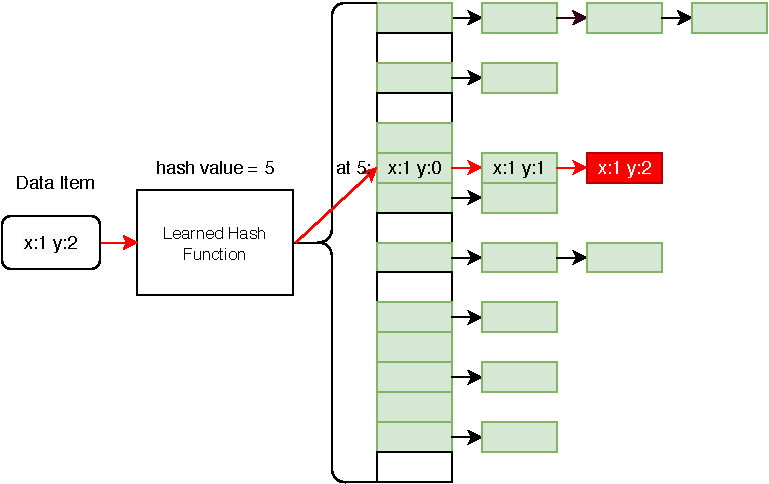
\includegraphics{Figures/hashmap.pdf}
\caption{The structure of the Learned Spatial Hashmap(LSPH). The search flow in LSPH takes one value from the selected dimension, then the learned hash function predicts the index to the estimated location in the hashmap.}
\label{fig:learned_spatial_hashmap}
}
\end{figure}

The Learned Spatial Hashmap(LSPH) is an efficient learned data index method for storing spatial data and handling spatial queries. The structure of the LSPH is straightforward, the main component of the index is a learned hashmap with chaining, as shown in Figure \ref{fig:learned_spatial_hashmap}. The learned hashmap is a hashmap with a learned CDF as its hash function \cite{Kraska:2017vh}. The CDF learned from a machine learning model and used it as a hash function in the hashmap. Linked lists are used in the LSPH for chaining. The design of the LSPH building process makes it suitable for storing spatial data points. The build process of the LSPH is shown as follows:

\begin{enumerate}
    \item \textbf{Dimension Selection}: Choosing one dimension from the dataset for model training.
    \item \textbf{Model Training}: A learned model trains on the selected dimension of data. 
    \item \textbf{Building of the LSPH}: Creating and Inserting to the Hashmap based on the prediction value.
\end{enumerate}

The learned model in LSPH trained only on a single dimension of two-dimensional data points. We select a single dimension of value from a coordinate data pair: $\{n|\forall n \in E.p\}$, where $E$ is every element in the dataset, and $p$ is selected dimension. The dimension selection is based on the  divergent of the values. A more divergent set of values can produce more divergent prediction values  from the same model. Therefore, it will optimize the loading factor of the hashmap, thus improving the efficiency of the lookup speed.

Using simple linear regression to train on data along a selected dimension $p$, with corresponding ranks of the data points, we can estimate a range of candidate positions of the query data point on the $p$ dimension, and trained model $m$. 

Memory with a size of the model prediction range will be allocated in the hashmap: $\hat{y}_{max} - \hat{y}_{min}$. The building process of the hashmap is relatively simple, the trained model $m$ inferences the input values from the same selected dimension $p$. Then the trained model yields a prediction value that can be treated as the hash value for the hashmap. Finally, the data point can be inserted into the hashmap at the index of the hash value. 

The LSPH is similar to a regular hashmap. It is simple but yet powerful. Some major differences distinguish itself from a regular hashmap, and suitable for storing and searching spatial objects. The LSPH uses only values from one dimension for the entire building procedure. Some properties about the learned hashmap guarantee the performance and accuracy of querying results, it will be discussed in the Section \ref{the_learned_hashmap}. 


\subsection{Single Dimensional Index Building}


\begin{figure}[ht]
\centering
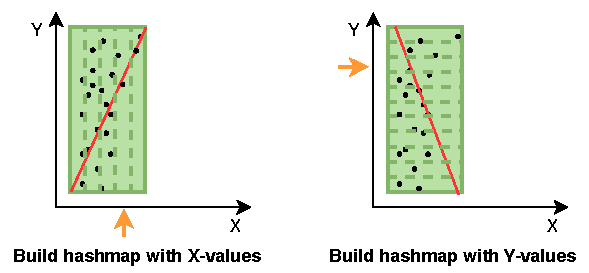
\includegraphics{Figures/single_dimension.pdf}
\caption{Difference between building data with x-values and y-values}
\label{fig:single_dimension}
\end{figure}

In the LSPH, the building process and the initial search range relies on one dimension of data. It is much easier to handle one-dimensional data than multidimensional data. The selection of the dimension for training is determined by the variance. Values on which dimension with a larger variance will be selected for model training. Given a series of two dimensional data $S = (x_i,\, y_i)$, compare the variance between $Var(x) \, \forall \, x \subseteq S$ and $Var(y) \, \forall \, y \subseteq S$, and dimension $p$ selected by the greater value between these two variances.


Transformation(space-filling curves, endpoint transformation and midpoint transformation) tends to be a popular choice for transferring multidimensional data into one-dimensional data in many traditional spatial indexes. In spatial data, it is hard to map two-dimensional data into one-dimensional data while preserving the spatial proximity \cite{Gaede:1998fp}. The space-filling curves (SFC) integrate both x-value and y-value into one value, to preserve the locality of points in the space. The calculated SFC values are used to rank the data points. Two closely-ranked data points in sorted order are also located close to each other in the spatial space. However, it requires extra calculations, and more importantly, a learned model can not produce an accurate prediction for the SFC values. 


There are some benefits for a spatial index to indexing from a single dimension of data. Training on a single dimension of values preserves the original information about the location, and it is already a one-dimensional data available. As a result, the LSPH has a fast query performance, since there is no pre-calculation for the transformation, values from original data can be used directly for inference. The building performance is also fast because of no extra calculation during the building process. 

Training on only a single dimension might also avoid potential data skewness. In most spatial datasets, skewness is most likely to happen in only one dimension. It means if one dimension is skewed, we can check if another dimension is skewed, and the training dimension $p$ is chosen from the less skewed out of two. Although there are some special cases, which values in both dimensions are skewed (such as two clusters of data points). It only creates computation overhead during searching in the chaining, and will not affect the accuracy of query results. 

 The selection of $p$ dimension can affect the space utility in the LSPH. A load factor in a hashmap is defined as: $\textit{Load Factor} = \frac{\textit{n}}{\textit{k}} $, where $n$ is \textit{number of entries occupied in the hashmap} and $k$ is \textit{size of hashmap}. The performance of the hashmap is largely decided by the load factor \cite{hashmap}. For example, a hashmap with a load factor of $0.5$ represents only half of the slots in the hashmap that are loaded with values. The hashmap in the LSPH is created with a size of prediction range, so in general, a high load factor can reduce chaining overhead and increase space utilization. For example, in Figure \ref{fig:single_dimension}, building the learned hashmap with y-values is much more efficient than building from x-values, because it can create more slots in the hashmap, and reduce the number of nodes in the linked list. As a result, the performance can also be improved from the reduction of computational overhead in lookup nodes from linked list chainings. 



\subsection{Learning a Hashmap} \label{the_learned_hashmap}


The learned hashmap has been mentioned in Kraska’s paper \cite{Kafle:2017dy}. He suggested that the learned hash map is no better than traditional hashmaps such as Cuckoo hashing in terms of solving conflict and distributing key mapping. There are some properties of the learned hashmap not mentioned in Kraska's paper, which can be strengths for handling spatial query operations. 

\textbf{Hashmap is a two-dimensional data structure}:
The hashtable and linked list chaining are two-dimensional, which is naturally suitable for routing two-dimensional data in those two components with values that belong to different dimensions. 


\textbf{Small hash collision rate}: According to Kraska, the learned hashmap can reduce hash conflict by up to 77\%. The logic behind it is that a randomized hash function is a trend to generate a random hash value, whereas the learned CDF can produce a hash value that grows with an increase of the input value. Therefore, it is less likely to have hash collisions with learned hash functions.

\textbf{Sorted head nodes}: Since the prediction results monotonically grow with the input value, the order of head nodes in the learned hashmap is sorted. In a set of sorted data, for any values $x\prime$ that are greater than a given input value $x$, the predicted value from the learned CDF function $y\prime = \text{CDF}(x\prime)$ is also greater than the predicted value $y = \text{CDF}(x)$. Kristo \cite{Kristo:2020it} implemented a sorting algorithm based on this property of the learned hashmap. 


\textbf{Load factor depends on model and data distribution}: The trained CDF maps all values from the dataset to the index value in the hashmap. Therefore, a good model choice and also the distribution of the data can affect the load factor. Whereas, the load factor in a hashmap that uses a random hash function is predetermined. This is critical to both memory space efficiency and query time performance. A high load factor can reduce the length of chaining to utilize the existing memory space in the hashmap, and also reduce the lookup overhead in the chaining. 

\textbf{Cost of hash function depends on the model}: Query performance also depends on the complexity of the learned model. In general, we want to have a model that can map the approximate distribution of data. However, if the model is complicated, then the query performance at inference can be affected. Rather, a high load factor in the hashmap is more important than having a computationally more expansive model for the query performance. 

\textbf{Guarantee to find value(completeness)}: Most learned indexes are attempting to search the position of the value key directly, but the prediction value always comes with an error bound. The model in LSPH does not predict the position of the index directly but is used as a hash value to access the position in the hashmap and potential chaining at that location. Therefore, the LSPH can guarantee to find the position of the key or the chaining where the key belongs to with one shot. 


Overall, these properties provide a foundation for the LSPH. The structure of the hashmap, monotonicity of head node and small collision rate are crucial for query accuracy, query performance and implementing spatial query algorithms. Compared to other learned indexes, the accuracy of a point query relies on the structure of the hashmap, rather than model prediction. Hence, the LSPH can guarantee the search result accuracy. 

\subsection{Model Choice}
The query performance is largely dependent on the model and the distribution of data. Because the prediction value is used as a hash value instead of the actual position of the key in the hashmap, the model does not need to be well fitted with the dataset. Neural networks are better for fitting data well, but it also takes a long time for training, and more expensive at inference. A linear model can do a good job, because the computation is much simpler. With a trained weight $w$ and bias $b$, linear function $y = wx \dot b$ can map an approximate distribution of data, and it can achieve a good performance at inference. Therefore, linear regression is chosen as the learned model for the LSPH, and the least square method is used for training the two parameters. As a result, the building process of LSPH is also fast. 


\section{Basic Operations}
The basic operations including insert, delete and update in the LSPH are also almost identical to a regular hashmap. Rather than changing the way a hashmap is used, we changed the data item content and made it suitable for handling spatial objects. Points in spatial space usually contain the coordinates of its location, which is ${x, y}$. As mentioned above, a dimension $p$ is chosen for model training, and it is also used for all operations of the LSPH. 


\begin{figure}[ht]
\centering
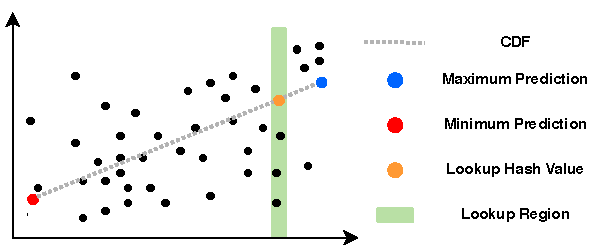
\includegraphics{Figures/search.pdf}
\caption{Lookup process on the dataset. Using the trained linear regression model to calculate the lookup hash value, then scanning the lookup region base on the lookup hash value.}
\label{fig:search}
\end{figure}


\textbf{Search}: Insertion and deletion heavily rely on searching data items in a data index. Searching an item in the LSPH requires hashing and chaining. $x-value$ or $y-value$ is chosen for hashing, based on the chosen $p$. A hash value is generated by the prediction value from the learned model: $h : V \rightarrow H$, where $H: \Leftrightarrow CDF$. The size of the LSPH is determined by the maximum and minimum prediction values: $m = \hat{y}_{max} - \hat{y}_{min}$, so when searching in the LSPH, the prediction value must subtract the minimum prediction value among the entire dataset to fit in the hashmap. The default rounding method to rounding from the float prediction value to integer is floor rounding. We found that rounding the closest integer can increase the variability of the resulting hash values, and raise the load factor. 

\textbf{Separate Chaining}: When a slot is occupied in the hashmap, the hash collision happens. A linked list will be created for chaining to solve the hash collision, any items that collided at the index in the hashmap will be appended to the end of the linked list. The length of the chaining is also determined by the load factor of the hashmap. Since the size of the hashmap is corresponding to the range of all prediction values, the higher the load factor is, the shorter the chaining will be. 

\textbf{Update}: To update an item, we need to determine whether the hash value of the data item is within the hashmap size of $m$. If the hash value is within the range, then we can insert the item as usual. If it is out of the range, the hashmap needs to be updated. The hash function model will be recalculated, and all existing items will be rehashed from the updated model. Since the linear model is used and the insertion process is relatively fast compared to neural network training, the rehash process is not considered expensive. 

\section{Query Processing}
The structure of LSPH adopted from the learned hashmap. What makes it able to manage spatial data is spatial query algorithms. Three types of spatial queries that are currently supported by LSPH: \textit{Point Query}, \textit{Range Query}, and \textit{k Nearest Neighbour query}. These three queries are focused on point object handling, but also developed a bounding box query algorithm that supports more complex spatial objects other than point objects.  

The most important and frequently executed operation is lookup a key. Key lookup in LSPH requires a hashing and iterative searching in the separate chaining. The performance of the lookup query is bounded by the length of chaining since the cost of hashing and indexing is always $O(1)$. The total cost of searching in the LSPH is $O(1 + \frac{n}{k})$, , where $\frac{n}{k}$ is the load factor. 

\subsection{Point Query}
\begin{algorithm}[H] \label{point_query}
\SetAlgoLined
\KwIn{Query point $q \ni {x_q, y_q}$}
\KwOut{Result query point $q_result$ that stored in the structure}
 $x\leftarrow{x_q}$, $y\leftarrow{y_q}$\;
 hashKey $\leftarrow{\text{hashFunc}(sort\_by\_x ? x : y)}$\;
 tempNode $\leftarrow{\text{table[hashkey]}}$\;
 \While{tempNode is not empty}{
  \eIf{tempNode.y $=$ y}{
    \If{tempNode.x $=$ x}
        {return tempNode\;}
   }{
   tempNode $\leftarrow{getNext()}$\;
  }
 }
 return null\;
 \caption{Point Query}
\end{algorithm}

The procedure of spatial point lookup consists of two parts: 
\begin{enumerate*}
    \item single dimensional value hashing
    \item local search in chaining.
\end{enumerate*}
 The steps are defined in Algorithm \ref{point_query}.

As described in previous sections, LSPH training used values on only one dimension. Therefore, a boolean variable $sort_by_x$, which is deducted from the single-dimensional index building,  is determining which dimension $p$ will be used in point lookup. Next, the selected value of $x$ will be hashed from a learned model. Since a linear model is mapping the approximate shape of the distribution of the dataset, the prediction/hash function is 
\begin{equation}
\hat{y} = x * w + b + 0.5f - (x<0)
\end{equation}
, where $0.5f - (x<0)$ is rounding float numbers to the closest integer value including negative numbers. Finally, a local iterative search is to find the actual position of the target tuple of spatial points, by comparing the value from another dimension and validate the selected value on $p$ dimension. 

The performance of the \textit{Point Query} is great for a uniformly distributed dataset since the querying process only requires one multiplication, one addition and local iteration with a size of  $\frac{n}{k}$. For all keys that share the same hash value will be placed in the same chaining. Therefore, the LSPH will guarantee to find the point. 


\subsection{Range Query}

\begin{figure}[ht]
\centering
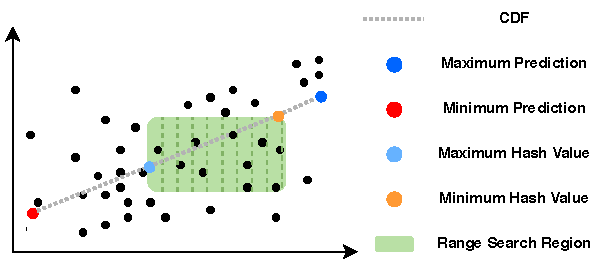
\includegraphics[scale=1]{Figures/range_search.pdf}
\caption{\textit{Range Query} in LSPH. Calculate the maximum and minimum hash value to get the search region on the hashmap.}
\label{fig:range_search}
\end{figure}


\textit{Range Query}, in addition to \textit{Point Query}, requires to specify the search range and scan through every data item if qualified. As illustrated in Figure \ref{fig:range_search}, first to find the $hashKeyMin$ and $hashKeyMax$ for the minimum and maximum x value, or minimum and maximum y value, depending on the $sort_by_x$. Then we can scan through every chain within the search region in the hashmap, to check if a data item from a node is in the searching range.


One of the properties of the monotonic growing learned map is that the values in the head nodes are sorted. Therefore, the $hashKeyMin$ and $hashKeyMax$ is defining the bounds of the search region. Any index value on the hashmap that exceeds the $hashKeyMin$ and $hashKeyMax$ will be out of the target region. At each chaining bucket, it just needs to check if points are within the range and if true then append the point to the result list. The time complexity for the range query depends on the size of the search region and the length of chaining.  

\begin{algorithm}[H] \label{range_query}
\SetAlgoLined
\KwIn{Range of search window $r$}
\KwOut{Set of result points $S$}
 $xMin, xMax, yMin, yMax\leftarrow{r}$\;
 $hashKeyMin = \text{hashFunc}(sort\_by\_x ? xMin : yMin)$\;
 $hashKeyMax = \text{hashFunc}(sort\_by\_x ? xMax : yMax)$\;
 $S\leftarrow{\emptyset}$\;
 \For{hashkey in from hashKeyMin to hashKeyMax}
 {
 tempNode $\leftarrow{\text{table[hashkey]}}$\;
    \While{tempNode is not empty}{
        \If{tempNode.x in $r$}
        {
            append tempNode to $S$\;
        }
        tempNode $\leftarrow{getNext()}$\;
    }
 }
 
 return $S$\;
 \caption{Range Query}
\end{algorithm}



\subsection{k Nearest Neighbours Query}

\begin{figure}[ht]
\centering
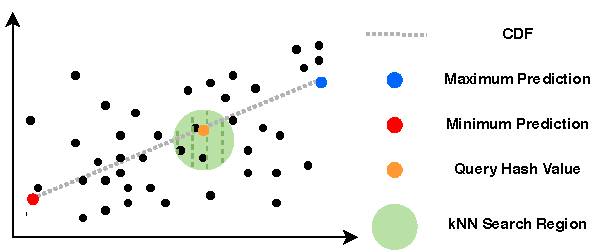
\includegraphics[scale=0.65]{Figures/knn.pdf}
\caption{\textit{kNN Query} in LSPH. First to calculate the query hash value, then expand to neighbour buckets.}
\label{fig:knn}
\end{figure}




The \textit{k Nearest Neighbours Query} finds $k$ number of point neighbours that have the closest distance to query point $q$. The algorithm starts with the same hashing process as in \textit{Point Query} and \textit{Range Query}. It first compares the distances with the current bucket of chaining, and stores the candidate into a priority queue that prioritizes based on the closest distance. Once it has been explored at the current index, it can expand the exploration to neighbour indexes. Since the indexes are sorted based on the monotonic growth of head nodes, the neighbour indexes are containing the closest nodes to the query node. Hence, the next step of the searching process will use two pointers, which one is doing an incremental search, and another one is doing a decremental search along the hashmap. The expansion search process will stop until the minimum of distances that collected at the current index is greater than or equal to the maximum distances collected previously.  Finally, k items pop out of the queue and return as the result of k nearest neighbours search

\begin{algorithm}[H] \label{knn_query}
\SetAlgoLined
\SetKwProg{Def}{def}{:}{}
\KwIn{Query point $q$; Number of nearest neighbours $k$}
\KwOut{Set of result points $S$}
$x\leftarrow{x_q}$, $y\leftarrow{y_q}$\;
hashKey $\leftarrow{\text{hashFunc}(sort\_by\_x ? x : y)}$\;
S $\leftarrow$ Priority Queue\;


% \tcp{Searching at current position in the table[hashKey]}

\Def{localSearch(hashKey)}{
    tempNode $\leftarrow{\text{table[hashKey]}}$\;
    \While{tempNode is not empty}{
        \If{$dist(tempNode, q) \leq minDist$}
            {append tempNode to S}
        tempNode $\leftarrow{getNext()}$\;
    }
}
% \tcp{ Search in current index is finished, starting search at expanding index in the table}

i $\leftarrow{hashKey+1}$; 
j $\leftarrow{hashKey-1}$\; 
previousMaxDist $\leftarrow{\text{S.Max()}}$;
localMinDist $\leftarrow{0}$\;
\While{localMinDist $<$ previousMaxDist}
 {
    previousMaxDist $\leftarrow$ previous S.Max()\;
    localSearch(i); localSearch(j)\;
    localMinDist $\leftarrow$ S.Min()\;
    i++; j--\,--\;
 }
 
 
 return $S$ with first k elements\;
 \caption{k Nearest Neighbours Query}
\end{algorithm}


The time complexity of Algorithm \ref{knn_query} is $O(1 + m\frac{n}{k})$, where $m$ is the size of expansion. Unlike hieratical structures such as B-Tree, the linear structure allows reducing redundant data scans caused by overlapping regions. Hence, LSPH can achieve more efficient kNN searching by fast hash computation and scanning regions reduction. 



\section{Minimum Bounding Box Handling}

\begin{figure}[ht]
\centering
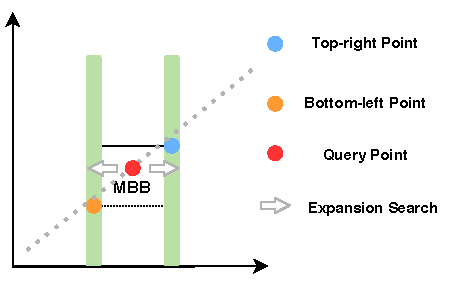
\includegraphics{Figures/object.pdf}
\caption{Store the top-right and bottom-right corners of a MBB in the hashmap}
\label{fig:object}
\end{figure}

The current process discussed above is all based on the point object in spatial data. We also implemented a method that allows the spatial index to handle more complex spatial objects such as line segments and polygons. All two-dimensional objects can be bounded by their minimum bounding box (MBB), which is a rectangle shape box defined by the minimum and maximum width and height of the object. The representation of MBB simplifies the structure of spatial objects. The $x$ and $y$ coordinate of two diagonal corner pointers are taken to store MBB in the LSPH.  

The fundamental operation of MBB supported by the LSPH is for a given query point $q$, the search result returns the MBB that the $q$ belongs to. To check if a point is within a particular MBB, both of the corner points need to be compared with the query point. Therefore, we have to insert both of the corner points of the same MBB into the LSPH. Each data item contains the $x$ and $y$ coordinate of the corresponding corner, and a pointer to extra information of the data item that contains coordinates from both corners. 

To retrieve the MBB from the query point, the procedure is similar to the k Nearest Neighbours Query: 
\begin{enumerate}
    \item Calculate the hash value from query point $q$.
    \item Search at the current index, which is the hash value.
    \item Iterative searching in the linked list at the current index. 
    \begin{enumerate}
        \item Retrieve coordinates of two corner pointers from data items in the linked list. 
        \item Check if the query point is within the currently searching MBB (defined by the two corner coordinates).
        \item If it is within the MBB region, return that MBB.  
    \end{enumerate}
    \item If no MBB found at the current index, expand the index to both sides (add and subtract the pointer). Repeat the search process.
\end{enumerate}

The performance of MBB searching is also similar to the performance of kNN query, except that MBB does not require a $k$ number of return values. Since we insert both the lower-left corner and upper-right corner into the hashmap, the searching pointer can compare to either corner arbitrarily. A pointer stores coordinate values of both corners are pointing to the hashmap item, so no matter which corner that the current searching pointer is comparing with, it can access the full information of both corners. 

There is one issue that can occur when two MBBs are overlapping, but the polygons themself do not overlap, the result will only return the first found MBB. To find the finer search result over polygon spatial objects, the information of the shape of the polygon is needed to calculate if the search point is within the polygon. 

\section{Summary}
Overall, the Learned Spatial Hashmap is a spatial index that applied model learning techniques. Although previous research has been carried out on learned models in spatial indexes, no single study has investigated applying learned hashmaps to handle spatial data. A large part of the study in this approach has devoted to the properties of learned hashmaps.  The property of a two-dimensional data structure is a natural side effect of chaining in a hashmap, which provides convenience for handling two-dimensional spatial data. The monotonic CDF is also an important feature in LSPH structure, which allows the inserted value to be sorted in the head node. Since the head nodes are sorted in the hashmap, consequently the support for range queries and KNN queries becomes easy. 

The LSHP is also flexible to choose one of two axes to train the CDF. Building a learned index from a selected dimension can utilize hashmap slot space, and reduce the length of the linked list. This simple technique not only increases the load factor of the hashmap, but it reduces the lookup time in the linked list as well. Therefore, the performance of LSHP can be optimized by selecting the right axis. 

In conclusion, LSHP is trying to balance the complexity of space and time. The search process finds a position of a key from a hashing function that only takes one multiplication and one addition and iterative search in the chaining linked list. The space complexity depends on the range of minimum and maximum prediction value, which is depending on the data distribution. Many learned indexes predict the position with an error bound. The benefit of this method is that it only needs to lookup keys in the disk page rather than store keys in the index structure. However,  they do not guarantee the accuracy of results 100\%. LSPH searches for the location of a query key based on the hash value, and a hash value is guaranteed to be the same from the same hash function. Therefore, as a tradeoff for memory, LSPH is guaranteed to have 100\% query accuracy. 

 % Experimental Setup

\chapter{Experiments}
In this section, I will discuss how I evaluate the LSH with some real world data, and comparison with other spatial indexes. Finally, present the outcome that is measured from various aspects.

\section{Experimental Setup}

For evaluation, the LSPH is implemented in C++ and has been tested on a machine with 2.2GHz 6-core Intel Core i7 CPU and 16GB memory. 

\begin{center}
\begin{adjustbox}{max width={\textwidth}, max totalheight={\textheight},keepaspectratio}
\begin{threeparttable}
\caption{Datasets}

\begin{tabular}{c|c c c}
    \toprule
                        % & \multicolumn{3}{c}{Dataset} \\\midrule \midrule
    \textbf{Name}    &\textbf{Size}  & \textbf{No. of data pairs} & \textbf{Data type}             \\ \midrule 
    \texttt{post}    & 2.2M & 123,593             &Geographic Coordinates \\
    \texttt{g2}      & 18K  & 2,048               & Synthetic Clusters    \\
    \texttt{osm}     & 3.0G & 114,932,854         &Geographic Coordinates \\
     \bottomrule
\end{tabular}
% \begin{tablenotes}
% \item[1] qwerty; \item[2] asdfgh
% \end{tablenotes}
\end{threeparttable}
\label{table:datasets}
\end{adjustbox}
\end{center}

\subsection{Datasets} 
As shown in the Table \ref{table:datasets} above, we have two real world datasets the \texttt{post} \cite{rtreeportal} and \texttt{osm} \cite{OpenStreetMap}, and one synthetic dataset the \texttt{g2} \cite{G2sets}. 

\begin{itemize}
  \item \texttt{post}: The \texttt{post} dataset contains 123,593 coordinates of post offices across North America. The distribution of this dataset is more evenly.
  \item \texttt{g2}: The \texttt{g2} is a synthetic cluster dataset that contains 2,048 points that are computed from Gaussian clusters with 2 dimensions and the standard deviation set to 10. 
  \item \texttt{osm}: The dataset \texttt{osm} contains 114,932,854 coordinates in Australia and Oceania from OpenStreetMap. This dataset contains large amount of data points, and its distribution is highly skewed. 
\end{itemize}


\begin{figure}
    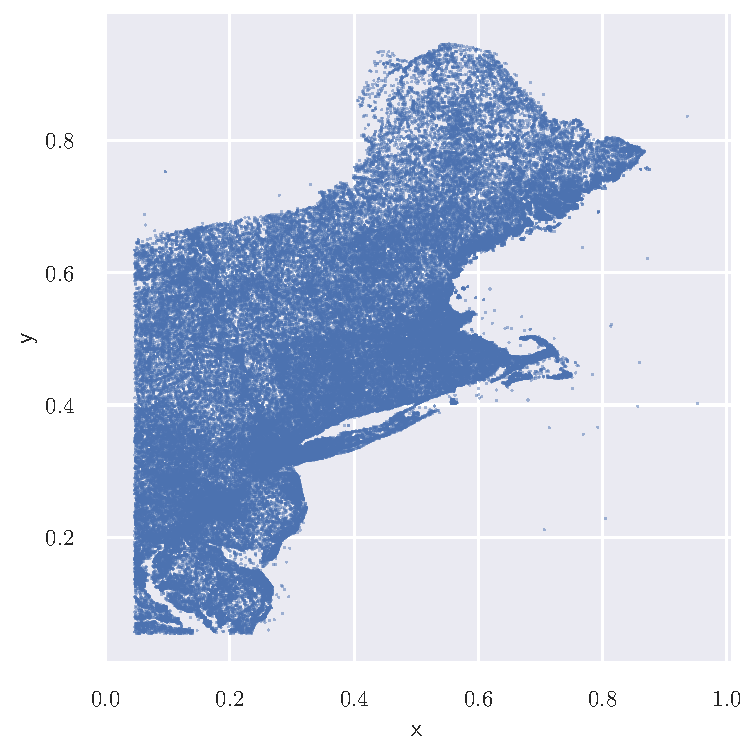
\includegraphics[width=.33\textwidth]{Figures/post_p.pdf}\hfill
    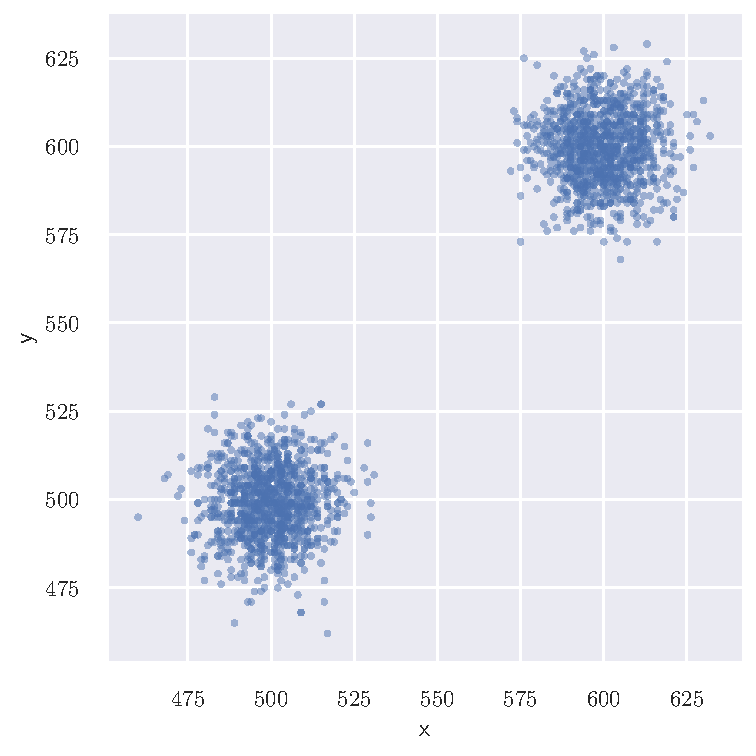
\includegraphics[width=.33\textwidth]{Figures/g2.pdf}\hfill
    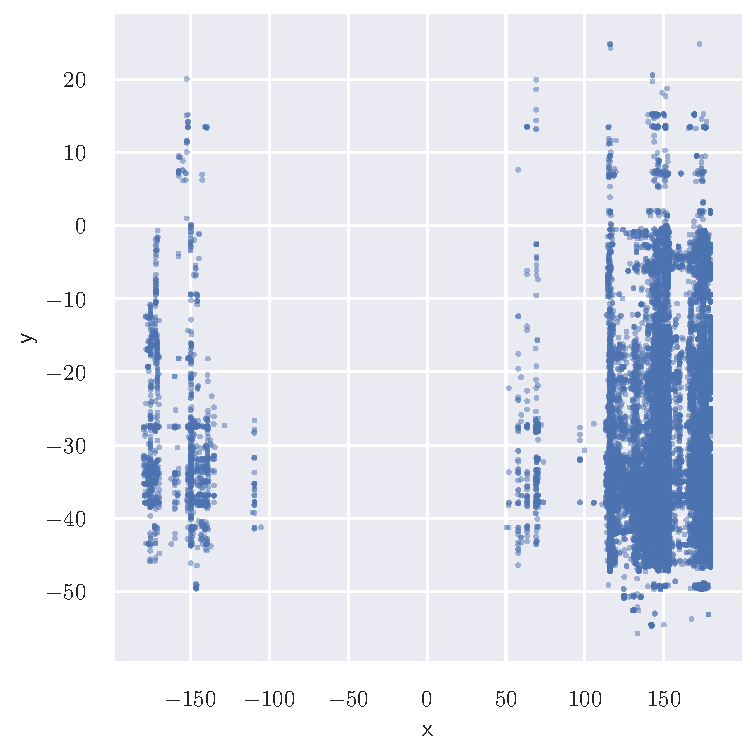
\includegraphics[width=.33\textwidth]{Figures/aus-ocean_p.pdf}
    \caption{Distribution of \texttt{post}, \texttt{g2} and \texttt{osm} datasets }\label{fig:datasets}
\end{figure}

Figure \ref{fig:datasets} illustrates the general size and distribution of each dataset. The three datasets represent three different data distribution settings: the post dataset has relatively uniform data distribution, and with over 100,000 data points making it common scenarios for spatial data indexing; the g2 is a synthetic two-dimensional dataset contains two clusters of data points, which is skewed on the both of axis, to test the skewness handling among the indexes; the osm is another real-world dataset with a sizable amount of data, and combine the heavily skewed data distribution, to test the performance under skewed high volume real-world scenario.  



\subsection{Competitors}
We are comparing LSPH with one traditional spatial index \textbf{R-Tree} \cite{Guttman:1984ka} and one learned spatial index \textbf{ZM} \cite{Wang:2019ks}

\textbf{R-Tree}: A templated C++ version implemented by Greg Douglas \cite{rtreecplus} is used for comparison. The partitioning method in this version uses the Quadratic-Cost splitting algorithm from the original R-Tree paper \cite{Guttman:1984ka}. 

\textbf{Learned ZM index}:  For the ZM model, the two-dimensional datasets convert to 64-bit one-dimensional data, using the Z-order curve transformation. We use an RMI implementation from the author of RadixSpline and SOSD \cite{Kipf:2020wr, sosd}. 

\subsection{Evaluation Metrics}
We measure the performance of all indexes from four aspects: memory consumption during runtime, time cost of index building, time cost of query and accuracy of the query result. The runtime memory reflects the space complexity of the index method, and the measurement is using the Linux command \texttt{time -v} to get the maximum resident set size of allocated memory size during runtime. Time measurements in the experiment were using the C++ \texttt{std::chrono} library to record the time during index building and query execution in nanoseconds. 

In the experiment, we use sorted arrays to build all indexes. Each index takes two data values as a pair of keys for lookup query, and if it exists in the index, the returned results should match with the query keys. We execute the lookup query overall key pairs in all three datasets. Note that there are some duplicates in the dataset, and they have been filtered out before indexes building. Therefore, the input number of the query should match with the returned results if the index can locate the key without errors. 



\section{Performance Results}

\begin{figure}
    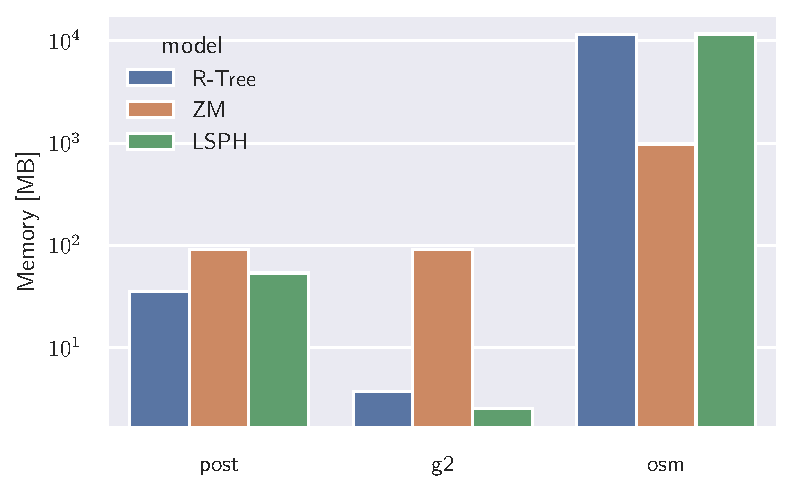
\includegraphics[width=.5\textwidth]{Figures/memory.pdf}\hfill
    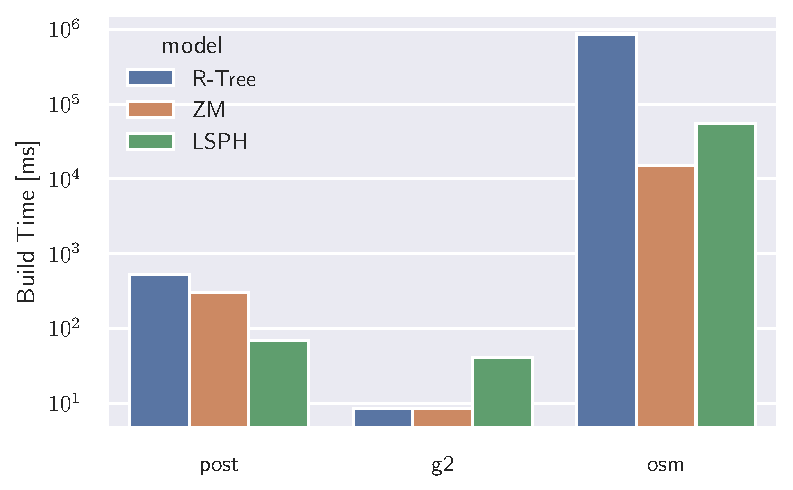
\includegraphics[width=.5\textwidth]{Figures/build_time.pdf}
    \\[\smallskipamount]
    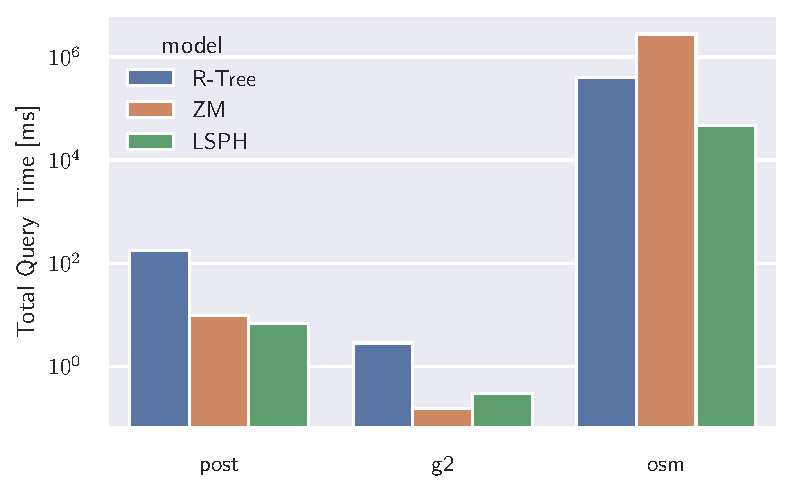
\includegraphics[width=.5\textwidth]{Figures/query_time.pdf}\hfill
    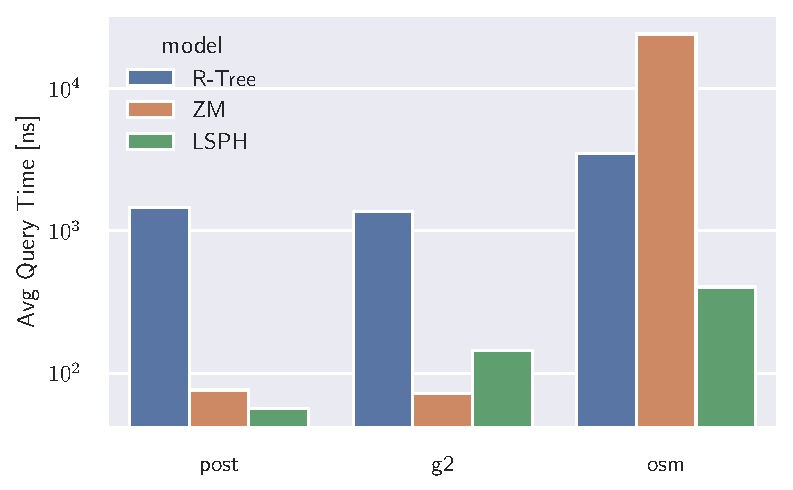
\includegraphics[width=.5\textwidth]{Figures/avg_query_time.pdf}
    \caption{Point query performance comparison on runtime memory, build time, total query time and average query time for all three spatial indexes}\label{fig:performance}
\end{figure}



\textbf{Overall performance}: We first compare the point query performance of all indexes on three datasets. Figure \ref{fig:performance} illustrates the overall performance of all indexes. The local search in the last step search in ZM used binary search, the total query time record the search range produced by a linear model plus the binary search execution time.  R-Tree uses minimum  bounding boxes to store all spatial objects. Therefore, for the point query in R-Tree, we set the minimum point and maximum point of a bounding box as the same pair of data values. As we see from the result, the LSPH has several advantages in memory and lookup query performance under certain conditions. 


\textbf{Runtime Memory}:
Comparing our method with R-Tree and ZM in terms of runtime memory consumption, as shown in the top-left diagram in Figure \ref{fig:performance}. LSPH consumes a similar amount of memory as R-Tree for all three sets of data. ZM costs more memory than LSPH and R-Tree in the \texttt{post} and \texttt{g2} dataset but costs less in the \texttt{osm} dataset. The ZM implementation requires running a rust code and converting it into C++ code, so it might consume more during conversion. The increase of numbers in the dataset causes a consistent growth in LSPH and R-Tree. For ZM, the memory cost is maintained at a certain level without concerning too much on the dataset size. 


\textbf{Build Time}: The build time of LSPH on a uniformly distributed dataset is outperforming the other two indexes. However, it cost more on skewed dataset \texttt{g2} and \texttt{osm}. Since we are using a linear model for the ZM, the build time is much faster than as if we were training a neural network. The reason for the slower build time of LSPH on the skewed dataset is that skewed data creates more chaining in the hashmap, which increases the node access during insertion. 



\textbf{Query Time}: Lookup query time showed a lookup performance advantage of LSPH. Note the log time scale in the total query time on the bottom of Figure \ref{fig:performance}, we also add an average query time for comparison. LSPH performed the best out of three indexes in the post and osm, and second place in the g2. The lookup speed in LSPH performs best in uniformly distributed datasets, it even can reach exact $O(1)$ if in a perfectly distributed dataset. The skewed data creates linked list overflow that causes some performance drop, but the average lookup speed is still kept at a slower growth compared to the ZM.  Although the lookup speed is much slower on an extreme cluster case where values on both axes are skewed, the LSPH still does a better job than ZM in terms of accuracy, which will be discussed in the next section.


\begin{center}
\begin{adjustbox}{max width={\textwidth}, max totalheight={\textheight},keepaspectratio}
\begin{threeparttable}
\caption{Point Query Accuracy}
\begin{tabular}{c|c c c}
    \toprule
                        % & \multicolumn{3}{c}{Dataset} \\\midrule \midrule
        &\textbf{R-Tree}  & \textbf{ZM} & \textbf{LSPH}             \\ \midrule 
    \texttt{post}    & 100\% & 99.99\% & 100\% \\
    \texttt{g2}      & 100\% & 99.71\% & 100\%  \\
    \texttt{osm}     & 100\% & 96.84\% & 100\% \\
     \bottomrule
\end{tabular}
% \begin{tablenotes}
% \item[1] qwerty; \item[2] asdfgh
% \end{tablenotes}
\end{threeparttable}
\label{table:accuracy}
\end{adjustbox}
\end{center}

\textbf{Accuracy}: Table \ref{table:accuracy} shows the accuracy of point query results from three indexes. R-Tree and LSPH can find every single query point from all three datasets. Some query points are not matching the query points in the ZM, due to the prediction positions are bounded by errors. If the errors have large ranges, for example, in the skewed datasets \texttt{g2} and \texttt{osm}, some predictions will exceed the maximum error ranges.


\subsection{Range Query Performance}

\begin{figure}
    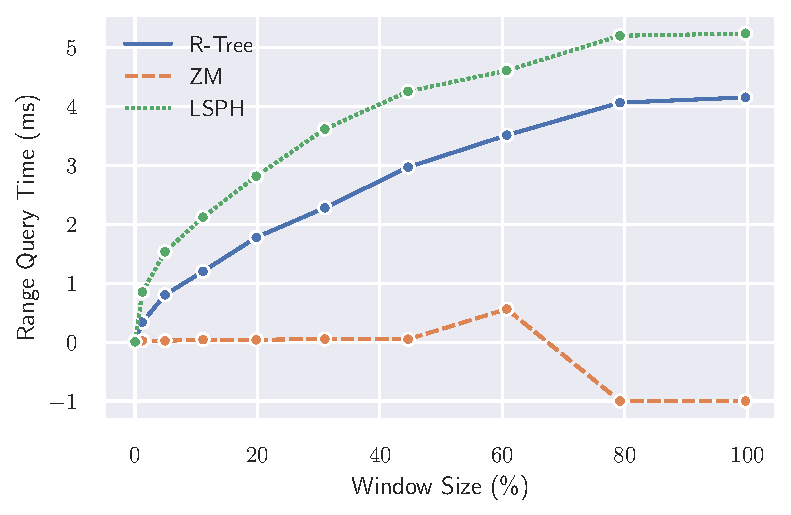
\includegraphics[width=\textwidth]{Figures/range_result.pdf}\hfill
    \caption{Range Query performance on dataset \texttt{post}. The window size is corresponding to the query selectivity, which is between 0.0-100.0\%. The -1 in ZM represents the return results are out of search range.}\label{fig:range_result}
\end{figure}

LSPH outperformed the other two indexes in point query speed. However, the range query can be considered as a weakness of the LSPH. The result is shown in Figure \ref{fig:range_result}. The range query performance was tested on the \texttt{post} dataset, since the \texttt{post} is more uniformly distributed that helps various window sizes can retrieve good amounts of data. The position of the range query window is located at the centre of the dataset, the selectivity of window size grows from 0 - 100 %.  

The performance of range queries of LSPH is worse than the R-Tree and the ZM. R-Tree is a hierarchical structure that its nodes contain the containment relationship between the minimum bounding box and spatial object. In range queries, the results are more likely to be found in the upper part of the tree, then check its child nodes. Therefore, R-Tree performed better at range query tasks. 

The overall performance of the ZM index is fast. However, in the last two window sizes 80\% and 100\%, the ZM can not retrieve points from the corresponding range, due to the predicted position being out of the maximum position. Hence, the ZM can not guarantee the accuracy of the search result. 

Our approach LSPH for the range query takes the longest time among the three. The range query algorithm in LSPH requires iterative search between a minimum hash value and a maximum hash value. However, it has to check every single point in the hashmap chaining. This means that the search is not only the head nodes in the hashmap but also every data item that is stored in the linked list. Therefore, it creates a lot of computational overhead. 


\subsection{Load Factor and Query Performance}

\begin{center}
\begin{adjustbox}{max width={\textwidth}, max totalheight={\textheight},keepaspectratio}
\begin{threeparttable}
\caption{load factor's effect on the query performance in LSPH}
\begin{tabular}{c|c c c}
    \toprule
                        % & \multicolumn{3}{c}{Dataset} \\\midrule \midrule
                                    &\texttt{post}      & \texttt{g2} & \texttt{osm}             \\ \midrule 
    \textbf{load factor}\tnote{1}            & 0.638\%   & 0.059\%   & 0.159\% \\
    \textbf{average query time}     & 52ns      & 155ns     & 403ns   \\
    \bottomrule
\end{tabular}
\begin{tablenotes}
\item[1] $\text{load factor} = \frac{n}{k}$, where n is the total number of entries, and k is the size of hashmap;
\end{tablenotes}
\end{threeparttable}
\label{table:loadfactor}
\end{adjustbox}
\end{center}

The load factor in the LSPH is dependent on data distribution and modelling. Comparing the load factors from all three datasets and their average query time is shown in the Figure \ref{table:loadfactor}. Overall, our statistics are consistent with the theoretical hypothesis that higher load factor in the hashmap will expect a better query performance. The \texttt{post} dataset has the best average query time with the highest load factor. The load factor in the \texttt{g2} is much lower than the load factor in the \texttt{osm}, but the average query time in the \texttt{g2} is still higher than the \texttt{osm}. The inconsistency of the result is because of differences between quantity of datasets. The \texttt{osm} contains significantly more data points then the \texttt{g2}, which takes more time in linked list search for LSPH. The load factor in \texttt{g2} is $10\times$ smaller than the load factor in \texttt{post}, and the average query time is $3\times$ slower than \texttt{post}. The load factor in \texttt{osm} is $4\times$ smaller than the load factor in \texttt{post}, and the average query time is $7.75\times$ slower than \texttt{post}.

Therefore, a higher load factor in the learned hashmap can achieve a better query performance. Besides the data distribution, models can also affect the load factor. Linear regression is great for mapping the approximate distribution of data and maintaining a very low computational cost. However, linear regression is not able to illustrate more complex curve shapes. It is worth considering piecewise monotonic regression in the future. 


\section{Summary}


 % Experiment 1

%\chapter{Conclusions and Future Work}
The primary objective of this study is to develop an understanding of learned spatial data indexes and propose a new approach of a spatial index with the learned model technique. Firstly, we have examined some previous works on the spatial data management techniques and spatial indexes based on that. We have also reviewed and compared some of the state-of-art learned one-dimensional indexes and learned spatial indexes. The conclusions obtained from the comparison suggest that a learned index model maps a data distribution that could potentially reduce the time complexity of query time, and as a benefit from directly locating the position of keys from models, the storage memory size of indexes is also lower than traditional data indexes. Notably, there are still some limitations in existing learning indexes. The RMI does not guarantee to find the query result 100\% accurately without hyperparameter tuning for a particular dataset. Lack of spatial query support in ZM and Flood also limit the functionalities of real-world application as a spatial data index. Neural network training in RMI, ZM and reinforcement learning in the qd-tree takes a long time to build, which can be a problem in real-world applications. 

Secondly, we proposed a new index method for handling spatial data and queries, the Learned Spatial Hashmap (LSPH). It integrates ideas that come from data science and machine learning to combine a learned CDF with a traditional hashmap. As a result of the learned CDF, the two-dimensional point query performance in LSPH achieved up to $8\times$ speedup compared to R-Tree and  $40\times$ speedup compared to ZM index.  The runtime memory cost of LSPH is similar to the R-Tree, which is overall balanced between space and time complexity. More importantly, LSPH addresses some disadvantages from existing learned model indexes. LSPH supports range queries, KNN queries, and can handle minimum bounding boxes. It is also worthwhile mentioning that LSPH guarantees query results to be 100\% accurate. 

\section{Limitations}
Our proposed spatial index method has a potential influence on studies in learned data indexes and real-world database applications. Folmer et al. \cite{Folmer:vg} proposed a Learning Spatial Buckets method for handling spatial data, which uses a similar idea of single dimension index building from our approach. However, there are not many studies that investigate the use of learned hashmap or other kinds of hashmap in the spatial index. Therefore, LSPH contributes a new idea to studies in spatial data management systems. 

LSPH provides the same result retrieving accuracy as the traditional spatial indexes and supports various spatial queries. LSPH has also been examined to outperform one of the popular traditional spatial data indexes and one of the state-of-art learned spatial indexes in real-world datasets.

It must also be mentioned that LSHP is still facing many challenges: 

\textbf{Skewness handling}: Notably, we have obtained a poor performance result from LSPH on the \texttt{g2} dataset. The single-dimensional index building has limitations when handling data skewness on both axes. Therefore, we would like to investigate the methods that can improve performance on skewed data. 

\textbf{Memory consumption}: LSHP might consume more memory in certain cases, because the size of the hashmap is determined by the minimum prediction value and the maximum prediction value, and even if there are very few data items between this prediction range, the hashmap will still allocate the same amount of slots. 

\textbf{Range query and KNN query performance}: Different from most spatial indexes, LSPH is a two-dimensional linear structure, rather than a hierarchical structure. The faster range query performance of the hierarchical structure indexes results from the containment relationship between parent nodes and child nodes. The KNN algorithm is also not very efficient by scanning the entire dataset. Future work is going to focus on building relationships between entries by experimenting with different structures and propose a more efficient KNN algorithm. 

\textbf{Model Choice}: Linear regression works well as the learned CDF in the hashmap. However, a major limitation of linear regression is it can not fit data distribution very well. Even the hashmap does not require a perfectly fitted CDF, but a more fitted model will result in better performance in terms of memory utilization and lookup speed. It is worth considering a piecewise linear function or interpolated polynomial model \cite{setiawan2020function}.

\section{Future Work}
Some of the issues listed from the limitations above are related to each other. Skewed data requires a more fitted model, and as a result of a more fitted model, the memory consumption can be reduced due to increase of hashmap load factor. We can investigate this problem from two aspects: model selection and data transformation. 

It is worth considering a piecewise linear function or interpolated polynomial model \cite{setiawan2020function}. Piecewise linear models have achieved good performance results from experiments in learned indexes such as PGM-index, FITing-index and Flood \cite{Ferragina:ud, galakatos2019fiting, Nathan:2019wc}. The piecewise linear model constructs a set of points and builds the segments of models according to the data range between two breakpoints. The resulting model learns the distribution of data better and differentiates the prediction values.  The interpolated polynomial model approximates the regression function from small training data. Such interpolated models generalize data better than linear regression, and it also requires much less time to train and less memory space compared to neural networks. 

Tsunami \cite{Ding:2020we} addresses data skewness problems from statistical tools: functional mapping and conditional CDFs to correlate skewed data. Functional mapping creates monotonically correlations between x values and y values. If the x value increases, the y value also increases in one direction. The transformed y values obtain a semantically linear relationship with the x values, so a linear regression function is enough for making predictions. Conditional CDFs maps x values dependent on the y values, in uniform $CDF(X|Y)$. Both methods are intended to construct a data correlation between two dimensions. 

Piecewise linear function and interpolated polynomial model or data correlation can both improve LSPH to handle skewed data better, and predict the accurate desired label values more effectively.  

In summary, LSPH contributes a new idea to the study of the learned multidimensional index, and improves the robustness and efficiency of spatial data management. Future work is going to focus on improving the skewed data handling in LSPH and exploring more to utilize the efficiency of LSPH.

 % Experiment 2

%\input{Chapters/Chapter6} % Results and Discussion

%\input{Chapters/Chapter7} % Conclusion

%% ----------------------------------------------------------------
% Now begin the Appendices, including them as separate files

% \addtocontents{toc}{\vspace{2em}} % Add a gap in the Contents, for aesthetics

% \appendix % Cue to tell LaTeX that the following 'chapters' are Appendices

% \chapter{An Appendix}

Lorem ipsum dolor sit amet, consectetur adipiscing elit. Vivamus at pulvinar nisi. Phasellus hendrerit, diam placerat interdum iaculis, mauris justo cursus risus, in viverra purus eros at ligula. Ut metus justo, consequat a tristique posuere, laoreet nec nibh. Etiam et scelerisque mauris. Phasellus vel massa magna. Ut non neque id tortor pharetra bibendum vitae sit amet nisi. Duis nec quam quam, sed euismod justo. Pellentesque eu tellus vitae ante tempus malesuada. Nunc accumsan, quam in congue consequat, lectus lectus dapibus erat, id aliquet urna neque at massa. Nulla facilisi. Morbi ullamcorper eleifend posuere. Donec libero leo, faucibus nec bibendum at, mattis et urna. Proin consectetur, nunc ut imperdiet lobortis, magna neque tincidunt lectus, id iaculis nisi justo id nibh. Pellentesque vel sem in erat vulputate faucibus molestie ut lorem.

Quisque tristique urna in lorem laoreet at laoreet quam congue. Donec dolor turpis, blandit non imperdiet aliquet, blandit et felis. In lorem nisi, pretium sit amet vestibulum sed, tempus et sem. Proin non ante turpis. Nulla imperdiet fringilla convallis. Vivamus vel bibendum nisl. Pellentesque justo lectus, molestie vel luctus sed, lobortis in libero. Nulla facilisi. Aliquam erat volutpat. Suspendisse vitae nunc nunc. Sed aliquet est suscipit sapien rhoncus non adipiscing nibh consequat. Aliquam metus urna, faucibus eu vulputate non, luctus eu justo.

Donec urna leo, vulputate vitae porta eu, vehicula blandit libero. Phasellus eget massa et leo condimentum mollis. Nullam molestie, justo at pellentesque vulputate, sapien velit ornare diam, nec gravida lacus augue non diam. Integer mattis lacus id libero ultrices sit amet mollis neque molestie. Integer ut leo eget mi volutpat congue. Vivamus sodales, turpis id venenatis placerat, tellus purus adipiscing magna, eu aliquam nibh dolor id nibh. Pellentesque habitant morbi tristique senectus et netus et malesuada fames ac turpis egestas. Sed cursus convallis quam nec vehicula. Sed vulputate neque eget odio fringilla ac sodales urna feugiat.

Phasellus nisi quam, volutpat non ullamcorper eget, congue fringilla leo. Cras et erat et nibh placerat commodo id ornare est. Nulla facilisi. Aenean pulvinar scelerisque eros eget interdum. Nunc pulvinar magna ut felis varius in hendrerit dolor accumsan. Nunc pellentesque magna quis magna bibendum non laoreet erat tincidunt. Nulla facilisi.

Duis eget massa sem, gravida interdum ipsum. Nulla nunc nisl, hendrerit sit amet commodo vel, varius id tellus. Lorem ipsum dolor sit amet, consectetur adipiscing elit. Nunc ac dolor est. Suspendisse ultrices tincidunt metus eget accumsan. Nullam facilisis, justo vitae convallis sollicitudin, eros augue malesuada metus, nec sagittis diam nibh ut sapien. Duis blandit lectus vitae lorem aliquam nec euismod nisi volutpat. Vestibulum ornare dictum tortor, at faucibus justo tempor non. Nulla facilisi. Cras non massa nunc, eget euismod purus. Nunc metus ipsum, euismod a consectetur vel, hendrerit nec nunc.	% Appendix Title

%\input{Appendices/AppendixB} % Appendix Title

%\input{Appendices/AppendixC} % Appendix Title

% \addtocontents{toc}{\vspace{2em}}  % Add a gap in the Contents, for aesthetics
\backmatter

%% ----------------------------------------------------------------
\label{Bibliography}
\lhead{\emph{Bibliography}}  % Change the left side page header to "Bibliography"
\bibliographystyle{ieeetr}  % Use the "unsrtnat" BibTeX style for formatting the Bibliography
\bibliography{Bibliography}  % The references (bibliography) information are stored in the file named "Bibliography.bib"

\end{document}  % The End
%% ----------------------------------------------------------------